\documentclass[12pt]{scrartcl}
%\usepackage{refcheck} 
\usepackage{a4}   
\usepackage{amsmath}    
\usepackage{paralist}
\usepackage{amssymb} 
\usepackage{amsfonts}  
\usepackage{mathrsfs}  
\usepackage{dsfont}
\usepackage{latexsym} 
\usepackage{xcolor}
\usepackage{bbm,exscale}
\definecolor{Myblue}{rgb}{0,0,0.6}  
\usepackage[colorlinks,citecolor=Myblue,linkcolor=Myblue,urlcolor=Myblue,pdfpagemode=None]{hyperref}
\usepackage{amsthm}
\usepackage{accents}
\usepackage[square,numbers,sort&compress]{natbib} 
\usepackage[all,cmtip]{xy}
\usepackage{ifthen} 
\usepackage{bbding}
\usepackage{stmaryrd}  
\usepackage{wasysym}
\usepackage{verbatim}
\usepackage{bbding} 
\usepackage{soul}  %allow linebreak for underlined with \ul
\usepackage[yyyymmdd,hhmmss]{datetime}
\usepackage{tikz}
\usepackage{tikz-cd}
\usepackage{tikz-3dplot}
\usepackage{pgfplots}
	\pgfplotsset{width=7cm,compat=1.8}
	%%External
%	 \usetikzlibrary{external}\tikzexternalize
%	\usetikzlibrary{decorations.pathmorphing}
%	\usetikzlibrary{decorations.pathreplacing}
	\usetikzlibrary{decorations.markings}
%	\usetikzlibrary{calc}
%	\usetikzlibrary{fadings}
%	\usetikzlibrary{matrix} 
	\usetikzlibrary{patterns}
%	\usetikzlibrary{shapes.geometric}
%	\usetikzlibrary{shadows}

%\pgfplotsset{compat=1.11}            
            

\tikzset{
    string/.style={draw=#1, postaction={decorate}, decoration={markings,mark=at position .51 with {\arrow[color=#1]{>}}}},
    costring/.style={draw=#1, postaction={decorate}, decoration={markings,mark=at position .51 with {\arrow[draw=#1]{<}}}},
    ostring/.style={draw=#1, postaction={decorate}, decoration={markings,mark=at position .47 with {\arrow[draw=#1]{>}}}},
    ustring/.style={draw=#1, postaction={decorate}, decoration={markings,mark=at position .56 with {\arrow[draw=#1]{>}}}},
    oostring/.style={draw=#1, postaction={decorate}, decoration={markings,mark=at position .43 with {\arrow[draw=#1]{>}}}},
    uustring/.style={draw=#1, postaction={decorate}, decoration={markings,mark=at position .59 with {\arrow[draw=#1]{>}}}},
    directed/.style={string=blue!50!black}, 
    odirected/.style={ostring=blue!50!black}, 
    udirected/.style={ustring=blue!50!black}, 
    oodirected/.style={oostring=blue!50!black}, 
    uudirected/.style={uustring=blue!50!black},     
    redirected/.style={costring= blue!50!black},
    redirectedgreen/.style={costring= green!50!black},
    directedgreen/.style={string= green!50!black},
    redirectedlightgreen/.style={costring= green!65!black},
    directedlightgreen/.style={string= green!65!black},
}

\tikzset{-dot-/.style={decoration={
  markings,
  mark=at position 0.5 with {\fill circle (1.875pt);}},postaction={decorate}}}

\tikzset{
	Fdot/.style={circle, draw, fill, inner sep=0pt}, 
	Odot/.style={circle, draw, inner sep=0.1pt, minimum size=0.1cm}
	}

\def\nicedashedcolourscheme{\shadedraw[top color=blue!22, bottom color=blue!22, draw=gray, dashed]}
\def\nicedashedpalecolourscheme{\shadedraw[top color=blue!12, bottom color=blue!12, draw=gray, dashed]}
\def\nicehalfpalecolourscheme{\shadedraw[top color=blue!22, bottom color=blue!22, draw=white]}
\def\nicenotpalecolourscheme{\shadedraw[top color=blue!32, bottom color=blue!32, draw=white]}
\def\nicecolourscheme{\shadedraw[top color=blue!22, bottom color=blue!22, draw=blue!22]}
\def\nicepalecolourscheme{\shadedraw[top color=blue!12, bottom color=blue!12, draw=white]}
\def\nicenocolourscheme{\shadedraw[top color=gray!2, bottom color=gray!25, draw=white]}
\def\nicereallynocolourscheme{\shadedraw[top color=white!2, bottom color=white!25, draw=white]}
\def\boringcolourscheme{\draw[fill=blue!20, dashed]}

\newcommand\tikzzbox[1]
%{pic}% 
{#1}%#1

  \tolerance 1414
  \hbadness 1414
  \hfuzz 0.3pt
  \widowpenalty=10000
  \vfuzz \hfuzz
  \raggedbottom
  
\makeatletter
\newcommand{\raisemath}[1]{\mathpalette{\raisem@th{#1}}}
\newcommand{\raisem@th}[3]{\raisebox{#1}{$#2#3$}}
\makeatother

\renewcommand{\H}{\mathcal H}
\newcommand{\Ccal}{\mathcal C}
\newcommand{\boldB}{\boldsymbol{B}}
\newcommand{\A}{\mathcal{A}}
\newcommand{\orb}{\mathcal{A}}
\newcommand{\sgn}{\mathrm{sgn}}
\renewcommand{\leq}{\leqslant}
\renewcommand{\geq}{\geqslant}

\newcommand{\E}{\text{e}} 
\newcommand{\I}{\text{i}}
\newcommand{\B}{\mathcal{B}}
\newcommand{\Borb}{\B_{\mathrm{orb}}}
\newcommand{\Beq}{\B_{\mathrm{eq}}}
\newcommand{\C}{\mathds{C}}
\newcommand{\D}{\mathds{D}}
\newcommand{\Ee}{\mathds{E}}
\newcommand{\K}{\mathds{K}}
\newcommand{\M}{\mathds{M}}
\newcommand{\N}{\mathds{N}}
\newcommand{\Q}{\mathds{Q}}
\newcommand{\R}{\mathds{R}}
\newcommand{\Z}{\mathds{Z}}
\newcommand{\IP}{\mathds{P}}
\def\1{\ifmmode\mathrm{1\!l}\else\mbox{\(\mathrm{1\!l}\)}\fi}
\newcommand{\one}{\mathbbm{1}}
\newcommand{\be}{\begin{equation}}
\newcommand{\ee}{\end{equation}}
\newcommand{\bes}{\begin{equation*}}
\newcommand{\ees}{\end{equation*}}
\newcommand{\cc}[1] {\overline{#1}}
\newcommand{\inv}[0]{{-1}}

\newcommand{\inver}[0]{\times}%{\mathrm{inv}}
\newcommand{\chirel}[0]{\chi_{\mathrm{sym}}}%{\chi_{\frac{1}{2}}}
\newcommand{\Dec}[0]{\mathrm{Dec}}
\newcommand{\interior}[1]{%
  {\kern0pt#1}^{\mathrm{o}}%
}
\newcommand{\Strat}[0]{\mathrm{Strat}}
\newcommand{\Stratdef}[0]{\mathrm{Strat}^{\mathrm{def}}}


\newcommand{\sVir}{\mathsf{sVir}}
\newcommand{\MF}{\operatorname{MF}_{\operatorname{bi}}}
\newcommand{\MFW}{\operatorname{MF}_{\operatorname{bi}}(W)}
\newcommand{\MFR}{\operatorname{MF}^\text{R}_{\operatorname{bi}}}
\newcommand{\DG}{\operatorname{DG}_{\operatorname{bi}}}
\newcommand{\DGW}{\operatorname{DG}_{\text{bi}}(W)}
\newcommand{\DGR}{\operatorname{DG}^\text{R}_{\text{bi}}}
\newcommand{\id}{\text{id}}
\newcommand{\KMF}{K_{0}(\operatorname{MF}_{\text{bi}}}
\newcommand{\Ext}{\operatorname{Ext}}
\newcommand{\Hom}{\operatorname{Hom}}
\newcommand{\End}{\operatorname{End}}
\newcommand{\modu}{\operatorname{mod}}
\def\LG{\mathcal{LG}}
\def\LGgr{\mathcal{LG}^{\mathrm{gr}}}
\def\LGgrs{\mathcal{LG}'^{\mathrm{gr}}}
\def\LGgrso{\mathcal{LG}'^{\mathrm{gr}}_{\mathrm{orb}}}
\def\LGs{\mathcal{LG}'}
\def\LGsorb{\mathcal{LG}'_{\mathrm{orb}}}
\def\LGorb{\mathcal{LG}_{\mathrm{orb}}}
\def\LGeq{\mathcal{LG}_{\mathrm{eq}}}
\newcommand{\hmf}{\operatorname{hmf}}
\newcommand{\HMF}{\operatorname{HMF}}
\newcommand{\ev}{\operatorname{ev}}
\newcommand{\eval}{\operatorname{eval}}
\newcommand{\tev}{\widetilde{\operatorname{ev}}}
\newcommand{\coev}{\operatorname{coev}}
\newcommand{\tcoev}{\widetilde{\operatorname{coev}}}
\def\lra{\longrightarrow}
% \def\lra{%
% \;%
% %%%%%%%%%%%%%%%%%%%%%% 
% \tikzzbox{\begin{tikzpicture}[scale=1.0,color=black, >=stealth, color=black, baseline=-0.1cm]
% \draw[-{stealth[length=1.6mm, scale width=1.1]}, line width=0.15mm] (0,0) -- (0.7,0);
% \end{tikzpicture}}%%popende
% %%%%%%%%%%%%%%%%%%%%%% 
% \;%
% }
\def\lmt{\longmapsto}
\DeclareMathOperator{\tr}{tr}
\DeclareMathOperator{\str}{str}
\DeclareMathOperator{\Jac}{Jac}
\def\Re{R^{\operatorname{e}}}
\DeclareMathOperator{\Res}{Res}
\newcommand*{\longhookrightarrow}{\ensuremath{\lhook\joinrel\relbar\joinrel\rightarrow}}
\newcommand*{\twoheadlongrightarrow}{\ensuremath{\relbar\joinrel\twoheadrightarrow}}
\newcommand{\Ga}[1]{\Gamma_{\hspace{-2pt}#1}}
\newcommand{\HIA}{\Hom(I,A)}
\newcommand{\ZA}{Z_A(\Hom(I,A))}
\newcommand{\gZA}{\!Z_A^\gamma(\Hom(I,A))}
\newcommand{\gA}{{}_{\gamma_A}A}
\newcommand{\Aginv}{A_{\gamma_A^{-1}}}
\newcommand{\picc}{\pi^{(\text{c,c})}_A}
\newcommand{\pirr}{\pi^{\text{RR}}_A}
\newcommand{\tpirr}{{\widetilde\pi}^{\text{RR}}} 
\newcommand{\im}{\operatorname{im}}
\DeclareMathOperator*{\eq}{=}
\DeclareMathOperator*{\congscript}{\cong}
\newcommand{\specflow}{\mathcal U_{-\frac{1}{2},-\frac{1}{2}}}
\newcommand{\Hil}{\mathcal{H}}
\newcommand{\Hpcc}{\mathcal{H}'_{\text{(c,c)}}}
\newcommand{\Hprr}{\mathcal{H}'_{\text{RR}}}
\newcommand{\Hcc}{\mathcal{H}_{\text{(c,c)}}^A}
\newcommand{\Hrr}{\mathcal{H}_{\text{RR}}^A}
\newcommand{\HccnoA}{\mathcal{H}_{\text{(c,c)}}}
\newcommand{\HrrnoA}{\mathcal{H}_{\text{RR}}}
\newcommand{\Hrrbo}{\Hom_A(X,{}_{\gamma_A}X)}
\newcommand{\buboorb}{\beta_X^{\text{orb}}}
\newcommand{\bobuorb}{\beta^X_{\text{orb}}} 
\def\Cong{C_g}
\def\Centg{N_g}
\def\alphaKK{\alpha^{\{K\}}}
\def\alphagKg{\alpha_g^{K(g)}}
\newcommand{\AGC}{A_G^c}

\newcommand{\Bord}{\operatorname{Bord}}
\newcommand{\Bordor}{\operatorname{Bord}_{n}^{\mathrm{or}}}
\newcommand{\Borddef}{\operatorname{Bord}^{\mathrm{def}}}
\newcommand{\Borddefn}[1] {\operatorname{Bord}^{\mathrm{def}}_{#1}}
\newcommand{\Bordoc}[1] {\operatorname{Bord}^{\mathrm{oc}}_{#1}}
\newcommand{\Bords}{\operatorname{Bord}_{3}^{\APLstar}}
\newcommand{\Sphere}{\operatorname{Sphere}^{\mathrm{def}}}
\newcommand{\Nbh}{\operatorname{\mathcal{N}}}
\newcommand{\Cube}{\operatorname{Cube}}
\newcommand{\Cubed}{\operatorname{Cube}_{3}^{\mathrm{def}}(\mathds{D})}
\newcommand{\Fradj}{\operatorname{\mathcal C_{\mathds D}^{adj}}}
\newcommand{\Bordstrat}{\operatorname{Bord}^{\mathrm{strat}}}
\newcommand{\Bordstratn}[1]  {\operatorname{Bord}^{\mathrm{strat}}_{#1}}
\newcommand{\Borddlong}{\operatorname{Bord}_{3}^{\mathrm{def}}(D_3,D_2,D_1)_{s,t,f}}
\newcommand{\Bordd[1]}{\operatorname{Bord}_{#1}^{\mathrm{def}}(\mathds{D})}
\newcommand{\Strator}{\operatorname{Strat}_{n}^{\mathrm{or}}}
\newcommand{\G}{\mathcal{G}}
\newcommand{\tz}{\mathcal T_\zz}
\newcommand{\dz}{\mathcal D_\zz}
\newcommand{\tzp}{\mathcal T_{\mathcal Z'}}
\newcommand{\Data}{\mathds{D}}
\newcommand{\Obj}{\mathrm{Obj}}
\newcommand{\zz}{\mathcal{Z}}
\newcommand{\Fdp}{\operatorname{\mathcal F}_{\textrm{d}}^{\textrm{p}}}
\newcommand{\zzd}{\mathcal{Z}^{\mathrm{def}}}
\newcommand{\zztriv}{\mathcal{Z}^{\mathrm{triv}}} 
\newcommand{\zzAtriv}{\mathcal{Z}_{\mathrm{triv}}^{\Cat{A}}} 
\newcommand{\euc}{\odot}
\newcommand{\euctwo}{\odot_{\geq 2}}
\newcommand{\ieuc}{\iota^\euc}
\newcommand{\peuc}{\pi^\euc}

\newcommand{\zzTVA}{\mathcal{Z}^{TV}_{\Cat{A}}} 
\newcommand{\zzRTC}{\mathcal{Z}^{RT}_{\Cat{C}}}
\newcommand{\tzztriv}{\mathcal{T}_{{\mathcal{Z}^{triv}}}}

\newcommand{\tzGamma}{\mathcal{T}_{{\mathcal{Z}^{\Gamma}}}}
\newcommand{\unit}{\operatorname{\mathbf{1}}}  
\newcommand{\bigslant}[2]{{\raisebox{.0em}{$#1$}\left/\raisebox{-.2em}{$#2$}\right.}}
\newcommand{\Cubedp}{\operatorname{Cube}_{3}^{\mathrm{def}}(\mathds{D}')}
\newcommand{\Borddp}{\operatorname{Bord}_{3}^{\mathrm{def}}(\mathds{D}')}
\newcommand{\Vect}{\operatorname{Vect}}
\newcommand{\Vectk}{\operatorname{Vect}_\Bbbk}
\newcommand{\Alg}{\operatorname{Alg}}
\newcommand{\Algc}{\operatorname{Alg}_{\C}}
\newcommand{\Cti}{\C^\times}
\newcommand{\chiom}{\chi^\omega}
\newcommand{\CGtw}{\C^\omega[G]}

\newcommand{\eps}{\varepsilon}
\newcommand{\al}{\alpha}
\newcommand{\alb}{\overline{\alpha}}
\newcommand{\T}{\mathcal{T}}
\newcommand{\Ss}{\mathcal{S}}
\newcommand{\X}{\mathcal{X}}
\newcommand{\Y}{\mathcal{Y}}
\newcommand{\sta}{\boxempty}
\newcommand{\fus}{\otimes}
\newcommand{\sd}{^{\star}}
\newcommand{\dagg}{^{\dagger}}
\newcommand{\hash}{^{\#}}
\newcommand{\Set}{\mathrm{Set}}
\newcommand{\Ball}{\mathrm{Ball}}
\newcommand{\Sph}{\mathsf{Sph}}
\newcommand{\fork}{\pitchfork }
\newcommand{\Cat}[1]         {\operatorname{\mathcal{#1}}}
\newcommand{\Catpre}[1]         {\operatorname{\mathcal{#1}^{\mathrm{pre}}}}

\newcommand{\dX}{{}^\dagger\hspace{-1.8pt}X}
\newcommand{\dA}{{}^\dagger\hspace{-1.8pt}A}
\newcommand{\dsX}{{}^\dagger\hspace{-1.8pt}\mathcal{X}}
\newcommand{\deqX}{{}^\star\hspace{-1.8pt}X} 
\newcommand{\dseqX}{{}^\star\hspace{-1.8pt}\mathcal{X}} 
\newcommand{\dY}{{}^\dagger\hspace{-0.3pt}Y}
\newcommand{\dphi}{{}^\dagger\hspace{-0.9pt}\phi}
\newcommand{\dPhi}{{}^\dagger\hspace{-0.9pt}\Phi}

%%%%%%%%%%%%%%%%%%%%%%%%%%%%%%%%%%%%%%%%%%%%%%%%%%%%%%%%%%%%%%%%%%%%%%%%%%%%%%%% 

\newcommand{\opp}             {{\mathrm{op}}} 

%\newcommand{\Alg}        {\operatorname{\mathsf{Alg}}}
\newcommand{\Frob}        {\operatorname{\mathsf{Frob}}}
\newcommand{\Lincat}        {\operatorname{\mathsf{Cat}^{ses}}}
\newcommand{\Deftqft}{\operatorname{TQFT}^{\mathrm{def}}}

\newcommand{\KVvect}   {\operatorname{KV-2Vect}}
\newcommand{\CYvect}   {\operatorname{CY-2Vect}}

\newcommand{\evx}[1]   {\operatorname{\mathsf{ev}}_{#1}}
% coevaluation
\newcommand{\coevx}[1]   {\operatorname{\mathsf{coev}}_{#1}}
% p evaluation
\newcommand{\evp}[1]   {\operatorname{\mathsf{ev}}_{#1}^{\prime}}
% p coevaluation
\newcommand{\coevp}[1]   {\operatorname{\mathsf{coev}}_{#1}^{\prime}}

\newcommand{\evc}[1]   {\operatorname{\mathsf{c-ev}}_{#1}}
% coevaluation
\newcommand{\coevc}[1]   {\operatorname{\mathsf{c-coev}}_{#1}}
% p evaluation
\newcommand{\evpc}[1]   {\operatorname{\mathsf{c-ev}}_{#1}^{\prime}}
% p coevaluation
\newcommand{\coevpc}[1]   {\operatorname{\mathsf{c-coev}}_{#1}^{\prime}}

\def\la               {{\rm l.a.}}
\def\ra               {{\rm r.a.}}
\def\rra              {{\rm r.r.a.}}
\def\lla               {{\rm l.l.a.}}
\def\Fun              {{\mathsf{Fun}}}
\def\Funbilin              {{\mathsf{Fun}^{\mathsf{bilin}}}}

\usepackage{color}

\newcommand{\rrr}[1]{{\color{red}{#1}}}
\newcommand{\rrR}[1]{{\color{red3}{#1}}}
\newcommand{\bbb}[1]{{\color{blue}{#1}}}
\definecolor{DarkViolet} {rgb}{0.580392,0.000000,0.827450}
\newcommand{\vio}[1]{{\color{DarkViolet}{#1}}}
\newcommand{\green}[1]{{\color{green}{#1}}}



\newcommand{\ques} [1] {\marginpar\textbf{qu}\textbf{{#1} ?}} 
\newcommand{\chn}[1]{\marginpar\textbf{changed}\textbf{{#1}}}
\newcommand{\note} [1] {\marginpar\textbf{note}\textbf{{#1}}}

\newcommand{\todo} [1] {\marginpar\textbf{todo} {\bbb{#1}  } }
\newcommand{\plan} [1] {\marginpar\textbf{Plan} { \bbb{#1}  } }
%comments
\newcommand{\GS} [1] {\marginpar{\small \vio{modified\\ by GS:} {}}{ \vio{#1} }} 
\newcommand{\GSC}[1] {\marginpar{\small \vio{comment \\ by GS:} {}}{ ~\\ \it \vio{#1} \\ }} 
\newcommand{\GSQ}[1] {\marginpar{\small \vio{question\\ by GS:} {}}{ ~\\ \it \vio{#1} \\ }} 
\newcommand{\IR} [1] {\marginpar{\small \rrr{modified\\ by IR:} {}}{ \rrr{#1} }} 
\newcommand{\IRC}[1] {\marginpar{\small \rrr{comment \\ by IR:} {}}{ ~\\ \it \rrr{#1} \\ }} 
\newcommand{\IRQ}[1] {\marginpar{\small \rrr{question\\ by IR:} {}}{ ~\\ \it \rrr{#1} \\ }} 
\newcommand{\NCMod} [1] {\marginpar{\small \vio{modified\\ by NC:} {}}{ \vio{#1} }} 
\newcommand{\NCC}[1] {\marginpar{\small \vio{comment \\ by NC:} {}}{ ~\\ \it \vio{#1} \\ }} 
\newcommand{\NCQ}[1] {\marginpar{\small \vio{question\\ by NC:} {}}{ ~\\ \it \vio{#1} \\ }} 

%%%%%%%%%%%%%%%%%%%%%%%%%%%%%%%%%%%%%%%%%%%%%%%%%%%%%%%%%%%%%%%%%%%%%%%%%%%%%%%% 



\newcommand\nxt{\noindent\raisebox{.08em}{\rule{.44em}{.44em}}\hspace{.4em}}
\newcommand\arxiv[2]      {\href{http://arXiv.org/abs/#1}{#2}}
\newcommand\doi[2]        {\href{http://dx.doi.org/#1}{#2}}
\newcommand\httpurl[2]    {\href{http://#1}{#2}}

\renewcommand{\labelenumi}{(\roman{enumi})}

\allowdisplaybreaks

\deffootnote[1em]{1em}{1em}{\textsuperscript{\thefootnotemark}}

\theoremstyle{definition}
\newtheorem{definition}{Definition}
\newtheorem{proposition}[definition]{Proposition}
\newtheorem{theorem}[definition]{Theorem}
\newtheorem{theoremdefinition}[definition]{Theorem and Definition}
\newtheorem{definitionlemma}[definition]{Definition and Lemma}
\newtheorem{lemma}[definition]{Lemma}
\newtheorem{corollary}[definition]{Corollary}
\newtheorem{remark}[definition]{Remark}
\newtheorem{remarks}[definition]{Remarks}
\newtheorem{conjecture}[definition]{Conjecture}
\newtheorem{example}[definition]{Example}
\newtheorem{construction}[definition]{Construction}

\numberwithin{equation}{section}
\numberwithin{definition}{section}
\numberwithin{figure}{section}

\newcommand\void[1]{}



\begin{document}

\title{Boundaries in finite gauge theory}

\author{%
\!\!\!\!\!\!\!Ilka Brunner \quad
Nils Carqueville \quad
Domenico Fiorenza \quad
}

\date{}
\maketitle

\tableofcontents



\section{Introduction}
\label{sec:intro}

Let 
\begin{itemize}
\item
$G$ be a finite group, 
\item
$\omega \in Z^n(G,\C^\times)$, 
\item
and $\Ccal$ a symmetric monoidal $(\infty,n)$-category for some $n\in \Z_+$.
\end{itemize}
On the one hand, \cite{FHLT} sketches the construction of a fullly extended TQFT
\be
\label{eq:TQFTfactored}
%%%%%%%%%%%%%%%%%%%%%%%
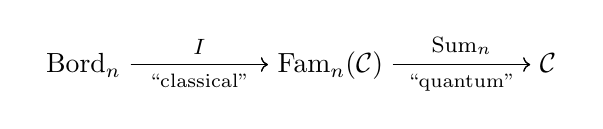
\begin{tikzpicture}[
			     baseline=(current bounding box.base), 
			     %>=stealth,
			     descr/.style={fill=white,inner sep=3.5pt}, 
			     normal line/.style={->}
			     ] 
\matrix (m) [matrix of math nodes, row sep=3.5em, column sep=5.0em, text height=1.5ex, text depth=0.1ex] {%
\Bord_n  &  \textrm{Fam}_n(\Ccal)  &  \Ccal 
\\
};
\path[font=\footnotesize] (m-1-1) edge[->] node[above] {$I$} (m-1-2);
\path[font=\scriptsize] (m-1-1) edge[->] node[below] {$\textrm{``classical''}$} (m-1-2);
\path[font=\footnotesize] (m-1-2) edge[->] node[above] {$\textrm{Sum}_n$} (m-1-3);
\path[font=\scriptsize] (m-1-2) edge[->] node[below] {$\textrm{``quantum''}$} (m-1-3);
\end{tikzpicture}
%%%%%%%%%%%%%%%%%%%%%%% 
\ee
based on the data $(G,\omega)$, which is viewed as a fully extended version of Dijkgraaf-Witten theory. 
On the other hand, in \cite{WittenParity2016, WWW} a class of boundary conditions for (classical!?) DW theory is proposed in terms of group extensions. 

\medskip

\noindent
\textbf{Goal. }
We want to reformulate the general aspects of the work \cite{WittenParity2016, WWW} in the setting of fully extended TQFT. 
More precisely, we view the bulk theories of \cite{WittenParity2016, WWW} as the classical part~$I$ in \eqref{eq:TQFTfactored} with $\Ccal = \boldB^n \C^\times$ (the $n$-fold delooping of the group~$\C^\times$) and then 
\begin{enumerate}
\item
identify \textsl{classical} boundary conditions as 1-morphisms with source $*$ in $\textrm{Fam}_n(\boldB^n \C^\times)$, 
\item
subsume the boundary conditions of \cite{WittenParity2016, WWW} as special cases, 
\item
map classical boundary conditions to quantum ones via $\textrm{Sum}_n$, and connect them to the known quantum boundary conditions, following the work of Ostrik and Fuchs--Schweigert--Valentino in the case $n=3$, 
\item 
do the above not only for framed, but also for oriented, spin,\dots TQFTs. 
\end{enumerate}

\medskip

Since \cite{FHLT} is very light on details, we first will work out explicitly how \eqref{eq:TQFTfactored} recovers the known bulk theory for $n \in \{1,2\}$ and hopefully also $n=3$. 
We also want to explain in detail how $(G,\omega)$ gives rise to an object in $\textrm{Fam}_n(\boldB^n \C^\times)$, and how group extensions $1 \to K \to H \stackrel{r}{\to} G \to 1$ give rise to 1-morphisms $\textrm{Fam}_n(\boldB^n \C^\times)(*, \boldB G)$. 
\\
(A more conceptual approach to boundary conditions and defects would be to start with a bordism category ``with singularities'' \cite[Sect.\,4.3]{l0905.0465} instead of $\Bord_n$, but we leave that for another project.)


\section{Special objects and 1-morphisms in $\textrm{Fam}_n(\boldB^n \C^\times)$}
\label{sec:FamBnC}

TODO: 
\begin{itemize}
\item 
spell out definition of $\textrm{Fam}_n(\Ccal)$
\item
check that $n$-functor $\boldB G \to \boldB^n \C^\times$ is precisely an $n$-cocycle
\\
\underline{\textbf{Issue}}: For $n>3$, what is a weak $n$-functor, i.\,e.~precisely what data and constraints are needed?
\\
\underline{\textbf{Idea}}: Since both $n$-categories in $\boldB G \to \boldB^n \C^\times$ are close to trivial, most data of the functor will be trivial, and the constraints (whatever they are) will be trivially satisfied. 
For $n \in \{1,2,3\}$ this is true, see Section~\ref{sec:bulk}. 
\item 
clarify precisely how $\boldB G \to \boldB^n \C^\times$ induces an $n$-functor $\boldB G \to n$-Vect, at least for $n \in \{1,2,3\}$
\item 
check whether natural transformation from trivial $n$-functor to $\omega \circ r$ is trivialisation of $r^* \omega$
\\
\underline{\textbf{Issue}}: induced from issue in second item
\end{itemize}


\subsection{Classical bulk theories}

TODO 

\subsection{Classical boundary conditions}

\subsubsection[$n=2$]{$\boldsymbol{n=2}$}

Let $\mathcal G_1, \mathcal G_2$ be 2-groupoids and let $F_1 \colon \mathcal G_1 \to \boldB^2\C^\times$ and $F_2 \colon \mathcal G_2 \to \boldB^2\C^\times$ be 2-functors, i.\,e.~objects in $\textrm{Fam}_2(\boldB^2 \C^\times)$. 
A 1-morphism $F_1\to F_2$ in $\textrm{Fam}_2(\boldB^2 \C^\times)$ is a span of 2-groupoids 
$
\mathcal G_1 \stackrel{K_1}{\longleftarrow} \widetilde{\mathcal G} \stackrel{K_2}{\lra} \mathcal G_2
$ 
together with a pseudonatural transformation $\sigma \colon F_1 \circ K_1 \to F_2 \circ K_2$: 
\be
%%%%%%%%%%%%%%%%%%%%%%%
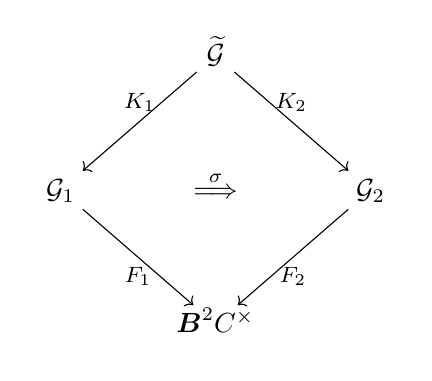
\begin{tikzpicture}[
			     baseline=(current bounding box.base), 
			     %>=stealth,
			     descr/.style={fill=white,inner sep=3.5pt}, 
			     normal line/.style={->}
			     ] 
\matrix (m) [matrix of math nodes, row sep=3.5em, column sep=3.0em, text height=1.5ex, text depth=0.1ex] {%
  &  \widetilde{\mathcal G}  &  
\\
\mathcal G_1 &  \stackrel{\sigma}{\implies}   &  \mathcal G_2
\\
  &  \boldB^2\C^\times  &  
\\
};
\path[font=\footnotesize] (m-1-2) edge[->] node[above] {$K_1$} (m-2-1);
\path[font=\footnotesize] (m-2-1) edge[->] node[below] {$F_1$} (m-3-2);
\path[font=\footnotesize] (m-1-2) edge[->] node[above] {$K_2$} (m-2-3);
\path[font=\footnotesize] (m-2-3) edge[->] node[below] {$F_2$} (m-3-2);
\end{tikzpicture}
%%%%%%%%%%%%%%%%%%%%%%% 
\ee

Let $[1]$ denote the final 2-category with only one object, 1- and 2-morphism, and let $T\colon [1] \to \boldB^2\C^\times$ be the unique, trivial 2-functor. 
A \textsl{classical boundary condition} for $F\colon \mathcal G \to \boldB^2\C^\times$ is a 1-morphism $T\to F$. 
Thus it comprises a 2-groupoid $\mathcal H$, a 2-functor $\rho \colon \mathcal H \to \mathcal G$, and a pseudonatural transformation 
\be
%%%%%%%%%%%%%%%%%%%%%%%
\begin{tikzpicture}[
			     baseline=(current bounding box.base), 
			     %>=stealth,
			     descr/.style={fill=white,inner sep=3.5pt}, 
			     normal line/.style={->}
			     ] 
\matrix (m) [matrix of math nodes, row sep=3.5em, column sep=3.0em, text height=1.5ex, text depth=0.1ex] {%
  &  \mathcal H  &  
\\
{[1]} &  \stackrel{\sigma}{\implies}   &  \mathcal G
\\
  &  \boldB^2\C^\times  &  
\\
};
\path[font=\footnotesize] (m-1-2) edge[->] node[above] {} (m-2-1);
\path[font=\footnotesize] (m-2-1) edge[->] node[below] {$T$} (m-3-2);
\path[font=\footnotesize] (m-1-2) edge[->] node[above] {$\rho$} (m-2-3);
\path[font=\footnotesize] (m-2-3) edge[->] node[below] {$F$} (m-3-2);
\end{tikzpicture}
%%%%%%%%%%%%%%%%%%%%%%% 
\ee
Concretely, since $\boldB^2\C^\times$ has only one object and one 1-morphism, $\sigma$ is given by a family of 2-morphisms $\sigma_h \colon (F\circ \rho)(h) = 1_* \to 1_*$, indexed by 1-morphisms~$h$ in~$\mathcal H$, such that
\be
%%%%%%%%%%%%%%%%%%%%%%%
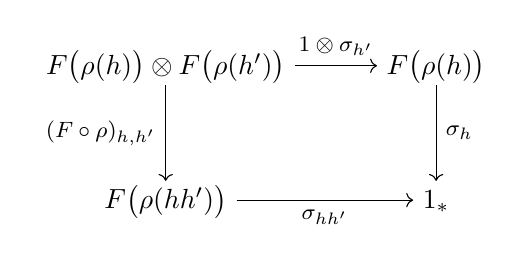
\begin{tikzpicture}[
			     baseline=(current bounding box.base), 
			     %>=stealth,
			     descr/.style={fill=white,inner sep=3.5pt}, 
			     normal line/.style={->}
			     ] 
\matrix (m) [matrix of math nodes, row sep=3.5em, column sep=3.0em, text height=1.5ex, text depth=0.1ex] {%
F\big(\rho(h)\big) \otimes F\big(\rho(h')\big)  &  F\big(\rho(h)\big)
\\
F\big(\rho(hh')\big)  & 1_*
\\
};
\path[font=\footnotesize] (m-1-1) edge[->] node[above] {$1\otimes \sigma_{h'}$} (m-1-2);
\path[font=\footnotesize] (m-1-1) edge[->] node[left] {$(F\circ\rho)_{h,h'}$} (m-2-1);
\path[font=\footnotesize] (m-2-1) edge[->] node[below] {$\sigma_{hh'}$} (m-2-2);
\path[font=\footnotesize] (m-1-2) edge[->] node[right] {$\sigma_{h}$} (m-2-2);
\end{tikzpicture}
%%%%%%%%%%%%%%%%%%%%%%% 
\ee
commutes for al composable 1-morphisms $h,h'$ in~$\mathcal H$. 

We now choose $\mathcal H = \boldB H$ for some finite group~$H$, $\mathcal G = \boldB G$, and $F = \chiom$ as in \eqref{eq:chiomega2} --- and we are not careful to distinguish the target $\boldB^2\C^\times$ from $\text{Alg}_\C$. 
Then a 2-functor $\rho \colon \boldB H \to \boldB G$ is just a group homomorphism $\rho \colon H \to G$, and a boundary condition 
\be
%%%%%%%%%%%%%%%%%%%%%%%
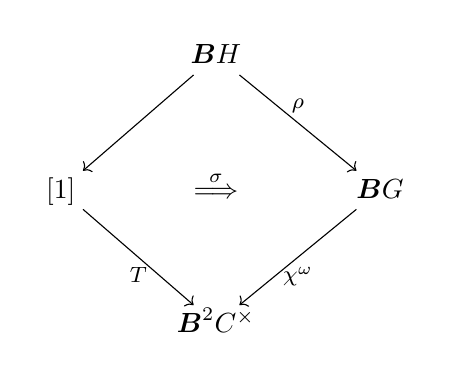
\begin{tikzpicture}[
			     baseline=(current bounding box.base), 
			     %>=stealth,
			     descr/.style={fill=white,inner sep=3.5pt}, 
			     normal line/.style={->}
			     ] 
\matrix (m) [matrix of math nodes, row sep=3.5em, column sep=3.0em, text height=1.5ex, text depth=0.1ex] {%
  &  \boldB H  &  
\\
{[1]} &  \stackrel{\sigma}{\implies}   &  \boldB G
\\
  &  \boldB^2\C^\times  &  
\\
};
\path[font=\footnotesize] (m-1-2) edge[->] node[above] {} (m-2-1);
\path[font=\footnotesize] (m-2-1) edge[->] node[below] {$T$} (m-3-2);
\path[font=\footnotesize] (m-1-2) edge[->] node[above] {$\rho$} (m-2-3);
\path[font=\footnotesize] (m-2-3) edge[->] node[below] {$\chiom$} (m-3-2);
\end{tikzpicture}
%%%%%%%%%%%%%%%%%%%%%%% 
\ee
for $\chiom$ is a family $\{ \sigma_h \}_{h\in H} \subset \C^\times$ such that 
\be
%%%%%%%%%%%%%%%%%%%%%%%
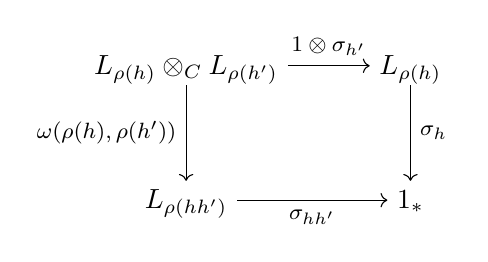
\begin{tikzpicture}[
			     baseline=(current bounding box.base), 
			     %>=stealth,
			     descr/.style={fill=white,inner sep=3.5pt}, 
			     normal line/.style={->}
			     ] 
\matrix (m) [matrix of math nodes, row sep=3.5em, column sep=3.0em, text height=1.5ex, text depth=0.1ex] {%
L_{\rho(h)} \otimes_\C L_{\rho(h')}  &  L_{\rho(h)}
\\
L_{\rho(hh')}   & 1_*
\\
};
\path[font=\footnotesize] (m-1-1) edge[->] node[above] {$1\otimes \sigma_{h'}$} (m-1-2);
\path[font=\footnotesize] (m-1-1) edge[->] node[left] {$\omega(\rho(h),\rho(h'))$} (m-2-1);
\path[font=\footnotesize] (m-2-1) edge[->] node[below] {$\sigma_{hh'}$} (m-2-2);
\path[font=\footnotesize] (m-1-2) edge[->] node[right] {$\sigma_{h}$} (m-2-2);
\end{tikzpicture}
%%%%%%%%%%%%%%%%%%%%%%% 
\ee
commutes, i.\,e.~$\omega(\rho(h),\rho(h')) = \sigma_h \cdot \sigma^{-1}_{hh'} \cdot \sigma_{h'}$ for all $h,h' \in H$. 
Viewing~$\sigma$ as a map $H\to \C^\times$, $h\mapsto \sigma_h$, this condition precisely means that~$\sigma$ trivialises the pullback of~$\omega$: 
\be
\textrm{d} \sigma = \rho^* \omega \, . 
\ee




\section{Bulk theory}
\label{sec:bulk}

\subsection[$n=1$]{$\boldsymbol{n=1}$}

Since we take the action of~$G$ on~$\C^\times$ to be trivial, the cocycle 
\be
\omega = [\omega] \in H^1(G,\C^\times) = \Hom_{\text{Grp}}(G,\C^\times)
\ee
is just a group homomorphism. 
We consider $\boldB^1 \C^\times$ as a subcategory of $\Vect_\C$, and we will use the pair $(G,\omega)$ to construct a functor
\be
\label{eq:TQFTfactored1}
%%%%%%%%%%%%%%%%%%%%%%%
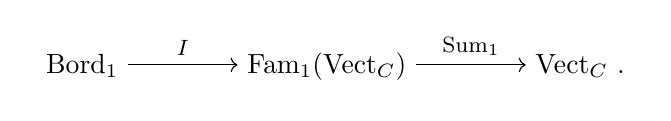
\begin{tikzpicture}[
			     baseline=(current bounding box.base), 
			     %>=stealth,
			     descr/.style={fill=white,inner sep=3.5pt}, 
			     normal line/.style={->}
			     ] 
\matrix (m) [matrix of math nodes, row sep=3.5em, column sep=4.0em, text height=1.5ex, text depth=0.1ex] {%
\Bord_1  &  \textrm{Fam}_1(\Vect_\C)  &  \Vect_\C \, . 
\\
};
\path[font=\footnotesize] (m-1-1) edge[->] node[above] {$I$} (m-1-2);
\path[font=\footnotesize] (m-1-2) edge[->] node[above] {$\textrm{Sum}_1$} (m-1-3);
\end{tikzpicture}
%%%%%%%%%%%%%%%%%%%%%%% 
\ee

According to the cobordism hypothesis, the composite $\textrm{Sum}_1 \circ I$ is determined by its value on the point $\text{pt}_+$, so we only need to specify $I(\text{pt}_+)$ and then compute $\textrm{Sum}_1(I(\text{pt}_+))$. 
Note that $\boldB^1 G = */\!\!/ G$ is the classical action groupoid. 
We set $I(\text{pt}_+)$ to be the functor
\be
\chi^\omega \colon */\!\!/ G \lra \Vect_\C 
\, , \qquad 
* \lmt \C
\, , \quad 
g \lmt \omega(g) \in \text{Aut}(\C)
\ee
%which sends~$*$ to~$\C$ and~$g$ to $\omega(g) \in \text{Aut}(\C)$ 
for all $g \in G$. 
Then \eqref{eq:TQFTfactored1} recovers the known result reviewed in \cite[Sect.\,1]{FHLT}: 

\begin{lemma}\label{lemma:cocone-is-coinvariants}
$\text{Sum}_1(\chi^\omega) = \C$ if $\omega(g) = 1$ for all $g\in G$, and $\text{Sum}_1(\chi^\omega) = 0$ otherwise. 
\end{lemma}

\begin{proof}
The statement is a particular case of this more general one: let $(V,\rho)$ be a linear representation of the group $G$, seen as the functor
\be
\chi^\rho \colon */\!\!/ G \lra \Vect_\C 
\, , \qquad 
* \lmt V
\, , \quad 
g \lmt \rho(g) \in \text{Aut}(V).
\ee
Then the universal cocone of $\chi^\rho$, viewed as a diagram of shape $*/\!\!/ G$ in $\Vect_\C$ is the pair $(V_G,\pi)$, where $V_G$ is the vector space of coinvariants for the representation $\rho$, i.e., 
\[
V_G=V/\langle v-\rho(g)v\rangle_{g\in G, v\in V}
\]
and $\pi\colon V\to V_G$ is the projection to the quotient. Namely, let $(W,f)$ be a cocone for $\chi^\rho$, i.e., a pair consisting of a vector space $W$ together with a linear map $f\colon \chi^\rho(*) = V \to W$ such that 
\be
%%%%%%%%%%%%%%%%%%%%%%%
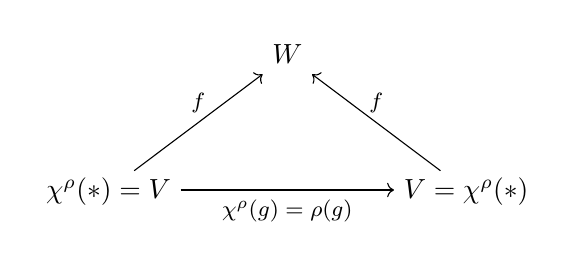
\begin{tikzpicture}[
			     baseline=(current bounding box.base), 
			     %>=stealth,
			     descr/.style={fill=white,inner sep=3.5pt}, 
			     normal line/.style={->}
			     ] 
\matrix (m) [matrix of math nodes, row sep=3.5em, column sep=3.0em, text height=1.5ex, text depth=0.1ex] {%
  &  W  &  
\\
\chi^\rho(*) = V &    &  V = \chi^\rho(*)
\\
};
\path[font=\footnotesize] (m-2-1) edge[->] node[above] {$f$} (m-1-2);
\path[font=\footnotesize] (m-2-1) edge[->] node[below] {$\chi^\rho(g) = \rho(g)$} (m-2-3);
\path[font=\footnotesize] (m-2-3) edge[->] node[above] {$f$} (m-1-2);
\end{tikzpicture}
%%%%%%%%%%%%%%%%%%%%%%% 
\ee
Then, by definition of $V_G$, the morphism $f$ uniquely factors through $V_G$ and so we have a commutative diagram
\be
%%%%%%%%%%%%%%%%%%%%%%%
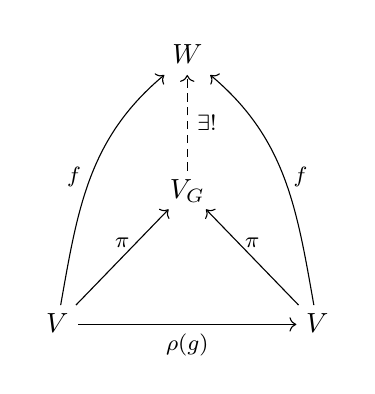
\begin{tikzpicture}[
			     baseline=(current bounding box.base), 
			     %>=stealth,
			     descr/.style={fill=white,inner sep=3.5pt}, 
			     normal line/.style={->}
			     ] 
\matrix (m) [matrix of math nodes, row sep=3.5em, column sep=3.0em, text height=1.5ex, text depth=0.1ex] {%
  &  W  &  
\\
  &  V_G  &  
\\
V  &    &  V
\\
};
\path[font=\footnotesize] (m-3-1) edge[->] node[above] {$\pi$} (m-2-2);
\path[font=\footnotesize] (m-3-1) edge[->] node[below] {$\rho(g)$} (m-3-3);
\path[font=\footnotesize] (m-3-3) edge[->] node[above] {$\pi$} (m-2-2);
%
\path[font=\footnotesize] (m-3-1) edge[->, out= 80, in= 220] node[left] {$f$} (m-1-2);
\path[font=\footnotesize] (m-3-3) edge[->, out= 100, in= -40] node[right] {$f$} (m-1-2);
%
\path[font=\footnotesize, densely dashed] (m-2-2) edge[->] node[right] {$\exists !$} (m-1-2);
\end{tikzpicture}
%%%%%%%%%%%%%%%%%%%%%%% 
\ee

%Hence $\text{Sum}_1(\chi^\omega)$ is in particular a cocone of $\chi^\omega$, i.\,e.~a vector space~$V$ together with a linear map $f\colon \chi^\omega(*) = \C \to V$ such that 
%\be
%%%%%%%%%%%%%%%%%%%%%%%%
%\begin{tikzpicture}[
%			     baseline=(current bounding box.base), 
%			     %>=stealth,
%			     descr/.style={fill=white,inner sep=3.5pt}, 
%			     normal line/.style={->}
%			     ] 
%\matrix (m) [matrix of math nodes, row sep=3.5em, column sep=3.0em, text height=1.5ex, text depth=0.1ex] {%
%  &  V  &  
%\\
%\chi^\omega(*) = \C  &    &  \C = \chi^\omega(*)
%\\
%};
%\path[font=\footnotesize] (m-2-1) edge[->] node[above] {$f$} (m-1-2);
%\path[font=\footnotesize] (m-2-1) edge[->] node[below] {$\chi^\omega(g) = \omega(g)$} (m-2-3);
%\path[font=\footnotesize] (m-2-3) edge[->] node[above] {$f$} (m-1-2);
%\end{tikzpicture}
%%%%%%%%%%%%%%%%%%%%%%%% 
%\ee
%commutes for all $g\in G$. 
%If $\omega(g) \neq 1$ for some~$g$, then this forces $f=0$, and the colimit is trivial: 
%\be
%%%%%%%%%%%%%%%%%%%%%%%%
%\begin{tikzpicture}[
%			     baseline=(current bounding box.base), 
%			     %>=stealth,
%			     descr/.style={fill=white,inner sep=3.5pt}, 
%			     normal line/.style={->}
%			     ] 
%\matrix (m) [matrix of math nodes, row sep=3.5em, column sep=3.0em, text height=1.5ex, text depth=0.1ex] {%
%  &  0  &  
%\\
%  &  V  &  
%\\
%\C  &    &  \C
%\\
%};
%\path[font=\footnotesize] (m-3-1) edge[->] node[above] {$f$} (m-2-2);
%\path[font=\footnotesize] (m-3-1) edge[->] node[below] {$\omega(g)$} (m-3-3);
%\path[font=\footnotesize] (m-3-3) edge[->] node[above] {$f$} (m-2-2);
%%
%\path[font=\footnotesize] (m-3-1) edge[->, out= 80, in= 220] node[left] {$0$} (m-1-2);
%\path[font=\footnotesize] (m-3-3) edge[->, out= 100, in= -40] node[right] {$0$} (m-1-2);
%%
%\path[font=\footnotesize, densely dashed] (m-2-2) edge[->] node[right] {$\exists !$} (m-1-2);
%\end{tikzpicture}
%%%%%%%%%%%%%%%%%%%%%%%% 
%\ee
%On the other hand, if~$\omega$ is trivial, every pair $(V,f)$ is a cocone, but the universal cocone is $(\C,1)$. 
showing that $(V_G,\pi)$ enjoys the universal property of the universal cocone.
\end{proof}

\begin{corollary}
The linear dual $\mathrm{Hom}_{\Vect_\C}(\text{Sum}_1(\chi^\omega),\C)$ of $\text{Sum}_1(\chi^\omega)$ is naturally isomorphic to the vector space of natural transformations $\mathrm{Hom}_{[*/\!\!/ G,\Vect_\C]}(\chi^\omega,\chi^1)$, where $\chi^1\colon  */\!\!/ G \to \Vect_\C$ is the trivial representation of $G$ on the vector space $\C$. In other words, we have
\[
\mathrm{Hom}_{\Vect_\C}(\text{Sum}_1(\chi^\omega),\C)\cong \left\{
\raisebox{40pt}{\xymatrix{
{*}/\!\!/ G\ar[dd]_{\chi^\omega}\ar[dr]\\
&{*}\ar[dl]^{\C}\\
\Vect_\C
\ar@{=>}(5,-13);(10,-13)
}}
\right\}.
\]
As a finite dimensional vector space is completely determined by its linear dual, this actually defines $\text{Sum}_1(\chi^\omega)$.
\end{corollary}
\begin{proof}
Again, the statement is true for an aritrary linear representation $(V,\rho)$ of the group $G$. The natural isomorphism
\[
\mathrm{Hom}_{\Vect_\C}(V_G,\C)\cong \left\{
\raisebox{40pt}{\xymatrix{
{*}/\!\!/ G\ar[dd]_{\chi^\rho}\ar[dr]\\
&{*}\ar[dl]^{\C}\\
\Vect_\C
\ar@{=>}(5,-13);(10,-13)
}}
\right\}
\]
is then nothing but the universal property of $V_G$. Namely, an element in the right hand side is a morphism $f\colon V=\chi^\rho(*)\to \chi^1(*)=\C$ such that all the diagrams
\[
\xymatrix{
V\ar[d]_{\rho(g)}\ar[r]^f & \C\ar[d]^{\mathrm{id}_\C}\\
V\ar[r]_f &\C
}
\]
commute, for any $g\in G$. This is the same as requiring that all the diagrams
\[
\xymatrix{
&\C\\
V\ar[rr]_{\rho(g)}\ar[ru]^{f} &&V\ar[lu]_{f}
}
\]
commute, and so it is precisely the datum of a morphism $V_G\to \C$ by the argumenti in the proof of Lemma \ref{lemma:cocone-is-coinvariants}.
\end{proof}


\subsubsection{Quantisation}

We now show that $\textrm{Sum}_1$ is a (TODO: symmetric monoidal!) functor. 

\medskip

Let us denote by $\mathrm{Fam}_0(\mathbb{C})$ the set of equivalence classes of finite groupoids equipped with functors to $\mathbb{C}$ (seen as a trivial category). In other words, a representative of an element of $\mathrm{Fam}_0(\mathbb{C})$ is a pair $(X,\rho)$ consisting of a finite groupoid $X$ together with a map $\rho\colon \pi_0(X)\to \mathbb{C}$.
The map 
\[
\mathrm{Sum}_0\colon \mathrm{Fam}_0\to \mathbb{C}
\]
is defined as
\[
\mathrm{Sum}_0(X,\rho)=\sum_{[x]\in \pi_0(X)}\frac{\rho(x)}{|\mathrm{Aut}(x)|}.
\]
We will also use the more evocative notation
\[
\int_X \rho(x) d\mu(x)
\]
to denote $\mathrm{Sum}_0(X,\rho)$. Notice that $\mathrm{Sum}_0$ is linear in the $\rho$ variable.

%The \textsl{mass} $\mu(X)$ of the finite groupoid $X$ is defined as
%\[
%\mu(X)=\mathrm{Sum}_0(X,1),
%\] 
%i.e., more explicitly,
%\[
%\mu(X)=\sum_{[x]\in \pi_0(X)}\frac{1}{|\mathrm{Aut}(x)|}.
%\]
A nice property of the morphism $\mathrm{Sum}_0$ (which we are going to use later) is the following: let $X$ be a finite set with an action of a finite group $G$, and let $X/\!/G$ denotes the action groupoid for this action; finally, let $\rho\colon X/\!/G\to \mathbb{C}$ any functor, i.e., let $\rho\colon X\to \mathbb{C}$ be a function that is constant on the $G$-orbits in $X$. Then we have
\begin{equation}\label{sum-0-on-action-groupoids}
\mathrm{Sum}_0(X/\!/G,\rho)=\frac{1}{|G|}\sum_{x\in X} \rho(x).
\end{equation}
Namely, the set $\pi_0(X/\!/G)$ is the quotient set $X/G$ and for any $x\in X$ seen as an object in $X/\!/G$ we have $\mathrm{Aut}(x)=\mathrm{Stab}_G(x)$. Therefore
\begin{align*}
\mathrm{Sum}_0(X/\!/G,\rho)&=\sum_{[x]\in X/G}\frac{\rho(x)}{|\mathrm{Stab}_G(x)|}\\
&=\frac{1}{|G|}\sum_{[x]\in X/G}\frac{|G|}{|\mathrm{Stab}_G(x)|}\rho(x)\\
&=\frac{1}{|G|}\sum_{[x]\in X/G}|[x]|\,\rho(x)\\
&=\frac{1}{|G|}\sum_{[x]\in X/G}\sum_{x\in [x]}\rho(x)\\
&=\frac{1}{|G|}\sum_{x\in X}\rho(x)
\end{align*}
\begin{remark}
A function $f\colon \pi_0(X)\to \mathbb{C}$ can equivalently be seen as an element in $\mathrm{End}_{[X,\mathrm{Vect}]}(\mathbf{1}_X)$, where $\mathbf{1}_X\colon X\to \mathrm{Vect}$ is the constant functor taking the value $\mathbb{C}$ on $X$. The map $\mathrm{Sum}_0$ can therefore be seen as the datum of a map
\[
\mathrm{Sum}_0\colon \mathrm{End}_{[X,\mathrm{Vect}]}(\mathbf{1}_X) \to \mathbb{C},
\]
for any finite groupoid $X$.
\end{remark}

\begin{definition}
The category $\mathrm{Fam}_1(\mathrm{Vect})$ has as its objects finite groupoids equipped with functors to $\mathrm{Vect}$, i.e., pairs $(X,\rho)$ consisting of a finite groupoid $X$ together with a functor $\rho\colon X\to \mathrm{Vect}$. Morphisms in $\mathrm{Fam}_1(\mathrm{Vect})$ are spans of groupoids over $\mathrm{Vect}$, i.e., commutative diagrams
\[
\xymatrix{
&Z\ar[dl]_{\pi_X}\ar[dr]^{\pi_Y}&\\
X\ar[dr]_{\rho_X}&&Y\ar[dl]^{\rho_Y}\\
&\mathrm{Vect}
\ar@{=>}_{\alpha\phantom{m}}(13,-14);(18,-14)
}
\]
where the natural transformation $\alpha\colon \rho_X\circ \pi_X\to \rho_Y\circ \pi_Y$ is part of the data of the commutative diagram.
\end{definition}
\begin{remark}
The identity mophisms and the composition of morphisms in $\mathrm{Fam}_1(\mathrm{Vect})$ will be defined later.
\end{remark}

For every object $(X,\rho)$ in $\mathrm{Fam}_1(\mathrm{Vect})$ we can consider the vector space 
\[
[\mathbf{1}_X,\rho]=\mathrm{Hom}_{[X,\mathrm{Vect}]}(\mathbf{1}_X,\rho).
\]
If $f\colon Y\to X$ is a functor between finite groupoids, and $\rho\colon X\to \mathrm{Vect}$ is a functor, we write $f^*\rho\colon Y\to \mathrm{Vect}$ for the functor $\rho\circ f$. If $\alpha\colon \mathbf{1}_X\to \rho$ is a natural transformation, then $f^*\alpha$ is a natural transformation between $f^*\mathbf{1}_X=\mathbf{1}_Y$ and $f^*\rho$. This defines a linear map
\[
f^* \colon [\mathbf{1}_X,\rho] \to [\mathbf{1}_Y, f^*\rho].
\]
Similarly, we can consider the vector space
\[
[\rho,\mathbf{1}_X]=\mathrm{Hom}_{[X,\mathrm{Vect}]}(\rho, \mathbf{1}_X)
\]
together with the linear map 
\[
f^* \colon [\rho,\mathbf{1}_X] \to [f^*\rho,\mathbf{1}_Y].
\]
Passing to the linear duals we get the linear map
\[
(f^*)^\vee\colon [f^*\rho,\mathbf{1}_Y]^\vee \to [\rho,\mathbf{1}_X]^\vee.
\]
Next, notice that composition of morphisms gives a bilinear map
\[
[\rho,\mathbf{1}_X]\otimes [\mathbf{1}_X,\rho] \to [\mathbf{1}_X,\mathbf{1}_X]
\]
and so composing this with the linear map $\mathrm{Sum}_0(X,-)\colon [\mathbf{1}_X,\mathbf{1}_X]\to \mathbb{C}$ we get a bilinear pairing $\langle\,|\,\rangle_X$ between $[\rho,\mathbf{1}_X]$ and $[\mathbf{1}_X,\rho]$, for any $\rho$. Notice that, by its very definition, the pairing $\langle\,|\,\rangle_X$ satisfies
\[
\langle v|\alpha\circ w\rangle_X =\langle  v\circ \alpha|w \rangle_X,
\]
for any $v\in [\rho_2,\mathbf{1}_X]$, any $w\in [\mathbf{1}_X,\rho_1]$ and any natural transformation $\alpha\colon \rho_1\to \rho_2$.
Equivalently, the bilinear pairing $\langle\,|\,\rangle_X$ is a linear map
\[
\delta_{(X,\rho)}\colon [\mathbf{1}_X,\rho]\to [\rho,\mathbf{1}_X]^\vee.
\]
Our main \textsl{duality assumption} will be that $\delta_{(X,\rho)}$ is a linear isomorphism for any $(X,\rho)$. 
\begin{remark}
The duality assumption holds for every finite groupoid $X$ if and only if it holds for finite connected groupoids. Up to equivalence we are therefore reduced to considering the case $X=\mathbf{B}G$, with $G$ a finite group. In this case $\rho\colon \mathbf{B}G\to \mathrm{Vect}$ is the datum of a linear representation $V$ of $G$, and the vector spaces $[\mathbf{1}_{\mathbf{B}G},\rho]$ and $[\rho,\mathbf{1}_{\mathbf{B}G}]$ are isomorphic to the space $V^G$ of $G$-invariants and the linear dual $(V_G)^\vee$ of the space of $G$-coinvariants, respectively. The map $\delta_{(\mathbf{B}G,\rho)}$ is therefore a map
\[
\delta_{(\mathbf{B}G,\rho)}\colon V^G\to (V_G)^{\vee\vee}\cong V_G,
\]
from $G$-invariants to $G$-coinvariants. Let $v\mapsto [v]$ be the canonical projection $V\to V_G=V/\langle v-g\cdot v\rangle_{v\in V;g\in G}$. By composing with the inclusion $V^G\hookrightarrow V$ we get the morphism $\iota\colon v\mapsto [v]$ from $V^G\to V_G$. This is an isomorphism. Indeed, the canonical projection $\pi\colon V\to V^G$ given by
\[
\pi\colon v\mapsto \frac{1}{|G|}\sum_{g\in G} g\cdot v
\]
is zero on the elements of the form $v-g\cdot v$ and so induces a linear map $\tilde{\pi}\colon V_G\to V^G$, which is immediate to see is the inverse of $\iota$.
For any $w\in (V_G)^\vee$ seen as an element in $[\rho,\mathbf{1}_{\mathbf{B}G}]$ and any $v\in V^G$ seen as an element in $[\mathbf{1}_{\mathbf{B}G},\rho]$ we have $w\circ v =w([v])$ Therefore
\[
\langle w| v\rangle_{\mathbf{B}G}=\frac{1}{|G|}w\circ v=w\left(\frac{1}{|G|}\iota(v)\right).
\]
This means that $\delta_{(\mathbf{B}G,\rho)}v$ is the evaluation on $\frac{1}{|G|}\iota(v)$. Therefore, under the canonical isomorphism $(V_G)^{\vee\vee}\cong V_G$, we have $\delta_{(\mathbf{B}G,\rho)}=\frac{1}{|G|}\iota$. As $\iota$ is an isomorphism, so is $\delta_{(\mathbf{B}G,\rho)}$.
\end{remark}

Under the duality assumption we may define a linear morphism 
\[
f_*\colon [\mathbf{1}_Y,f^*\rho]\to  [\mathbf{1}_X,\rho]
\]
as the composition
\[
[\mathbf{1}_Y,f^*\rho]\xrightarrow{\delta_{(Y,f^*\rho)}}[f^*\rho,\mathbf{1}_Y]^\vee \xrightarrow{(f^*)^\vee} [\rho,\mathbf{1}_X]^\vee \xrightarrow{\delta_{(X,\rho)}^{-1}} [\mathbf{1}_X,\rho].
\]
In other words, if $v\in [\mathbf{1}_Y,f^*\rho]$, the element $f_*v\in [\mathbf{1}_X,\rho]$ is defined 
%by the equation
%\[
%\int_X (w\circ f_*(v)) d\mu(x) = \int_Y((f^*w)\circ v) d\mu(y),
%\]
%i.e.,
 by the equation
\[
\langle w| f_*v\rangle_X = \langle f^*w| v\rangle_Y
\]
for any $w\in [\rho,\mathbf{1}_X]$. Similarly, we have a morphism $f_*\colon [f^*\rho,\mathbf{1}_Y]\to [\rho,\mathbf{1}_X]$ defined by
\[
\langle f_*w| v\rangle_X = \langle w| f^*v\rangle_Y.
\]

For  later use, let us derive an explicit formla for $f_*$ in case $f\colon \mathbf{B}G\to \mathbf{B}H$ is a morphism of finite groups (seen as groupoids with a single object).

\begin{lemma}
\label{lem:pushonBG}
If $G,H$ are finite groups and $f\colon \mathbf{B}G\to \mathbf{B}H$ is a functor, then for every $v\in [\mathbf{1}_{\mathbf{B}G},f^*\rho]$ we have 
$$
f_*v=\frac{1}{|G|}\sum_{h\in H} h\cdot v \, . 
$$
\end{lemma}

\begin{proof}
Recall that  if $v\in [\mathbf{1}_{\mathbf{B}G},f^*\rho]$, the element $f_*v\in [\mathbf{1}_{\mathbf{B}H},\rho]$ is defined by the equation $\langle w| f_*v\rangle_{\mathbf{B}H} = \langle f^*w| v\rangle_{\mathbf{B}G}$
for any $w\in [\rho,\mathbf{1}_{\mathbf{B}H}]$. As both $\mathbf{B}G$ and $\mathbf{B}H$ have a single object, this equation reduces to
\[
\frac{w\circ f_*v}{|H|}=\frac{f^*w\circ v}{|G|}
\] 
The morphism $\rho\colon \mathbf{B}H\to \mathrm{Vect}$ is the datum of a linear representation of $H$ on a vector space $V$, and $f^*\rho$ is the datum of representation of $G$ obtained by pull-back, i.e., the group $G$ acts on $V$ by $g\cdot \xi := f(g)\cdot \xi$. The element $v\in [\mathbf{1}_{\mathbf{B}G},f^*\rho]$ is therefore a $G$-invariant vector of $V$, while $w\in [\rho,\mathbf{1}_{\mathbf{B}H}]$ is a linear functional on $V$ factoring through the space of $H$-coinvariants. The element $f^*w$ is the same linear functional on $V$, but this time seen as factoring through the space of $G$-coinvariants. Therefore the composition $f^*w\circ v$ is just the evaluation of $w\colon V\to \mathbb{C}$ on the vector $v\in V$, under the canonical isomorphism $\mathrm{End}(\mathbb{C})\cong \mathbb{C}$. Finally, $f_*v\in  [\mathbf{1}_{\mathbf{B}H},\rho]$ is an $H$-invariant vector of $V$, and $w\circ f_*v$ is the evaluation of $w\colon V\to \mathbb{C}$ on the vector $f_*v\in V$. The defining equation for $f_*v$ then becomes
\[
w\left(\frac{f_*v}{|H|}\right)=w\left(\frac{v}{|G|}\right)
\] 
for any $w\colon V\to \mathbb{C}$ factoring through the space of $H$-coinvariants.
From $v/|G|$ we get the $H$-invariant vector 
\[
\frac{1}{|H|}\sum_{h\in H}h\cdot \frac{v}{|G|}
\]
and, since $w$ factors through the $H$-coinvariants,
\[
w\left(\frac{v}{|G|}\right)=w\left(\frac{1}{|H|}\sum_{h\in H}h\cdot \frac{v}{|G|}\right)
\]
The defining equation for $f_*v$ can therefore be rewritten as
\[
\langle w| f_*v\rangle_{\mathbf{B}H}=\langle w| \sum_{h\in H}\frac{h\cdot v}{|G|}\rangle_{\mathbf{B}H},
\]
for any $w\in [\rho,\mathbf{1}_X]$. As the pairing $\langle \,| \,\rangle_{\mathbf{B}H}$ is nondegenerate, this finally gives
\[
f_*v=\frac{1}{|G|}\sum_{h\in H} h\cdot v.
\] 
\end{proof}

\begin{remark}
This formula simplifies a bit in case the group homomorphism $f\colon G\to H$ is surjective. Indeed, in that case, the $G$-invariant vector $v$ will be automatically $H$-invariant and we find
\[
f_*v=\frac{|H|}{|G|} v
\]
in this case.
\end{remark}

We can now define our wannabe functor
\[
\mathrm{Sum}_1\colon \mathrm{Fam}_1(\mathrm{Vect})\to \mathrm{Vect}
\]
on objects as 
\[
\mathrm{Sum}_1(X,\rho)=[\mathbf{1}_X,\rho]
\]
and on a morphism 
\[
\xymatrix{
&Z\ar[dl]_{\pi_X}\ar[dr]^{\pi_Y}&\\
X\ar[dr]_{\rho_X}&&Y\ar[dl]^{\rho_Y}\\
&\mathrm{Vect}
\ar@{=>}_{\alpha\phantom{m}}(13,-14);(18,-14)
}
\]
as the composition
\[
[\mathbf{1}_X,\rho_X]\xrightarrow{\pi_X^*} [\mathbf{1}_Z,\pi_X^*\rho_X]\xrightarrow{\alpha\circ-}  [\mathbf{1}_Z,\pi_Y^*\rho_Y] \xrightarrow{\pi_{Y*}} [\mathbf{1}_Y,\rho_Y].
\]

\begin{remark}
Before giving a more explicit expression of the above morphism, let us notice that $[\mathbf{1}_X,\rho]$ is a model for the limit of the functor $\rho\colon X\to \mathrm{Vect}$, in accordance with the prescription in \cite{FHLT}. Also, notice that the morphism associated to the span $X\leftarrow Z\to Y$ together with the natural transformation $\alpha$ has the form ``pull-compose-push'', and so it is an instance of a Fourier-Mukai-type transform.
\end{remark}



\begin{lemma} (The projection formula)
\label{lem:projectionformula}
Let $f\colon Y\to X$ be a functor between finite groupoids, let $\rho_1,\rho_2\colon X\to \mathrm{Vect}$ be functors and let $\alpha\colon \rho_1\to\rho_2$ be a natural transformation. We have an identity of morphisms $[\mathbf{1}_Y,f^*\rho_1]\to [\mathbf{1}_X,\rho_2]$
\[
f_*(f^*\alpha\circ -) = \alpha\circ f_*
\] 
\end{lemma}
\begin{proof}
The identity
\[
f_*(f^*\alpha\circ v) = \alpha\circ f_*v
\]
for every $v\in [\mathbf{1}_Y,f^*\rho_1]$ is equivalent to the identity
\[
\langle w| f_*(f^*\alpha\circ v)\rangle_X = \langle w|\alpha\circ f_*v\rangle_X
\]
for every $v\in [\mathbf{1}_Y,f^*\rho_1]$ and every $w\in [\rho_2,\mathbf{1}_X]$. By the properties of the pairings $\langle\,|\,\rangle_X$ and $\langle\,|\,\rangle_Y$, and by definition of $f_*$, we have
\begin{align*}
\langle w| f_*(f^*\alpha\circ v)\rangle_X&=\langle f^*w| f^*\alpha\circ v\rangle_Y\\
&=\langle f^*w\circ f^*\alpha| v\rangle_Y\\
&=\langle f^*(w\circ \alpha)| v\rangle_Y\\
&=\langle w\circ \alpha| f_*v\rangle_X\\
&=\langle w| \alpha \circ f_*v\rangle_X
\end{align*}
\end{proof}

\begin{lemma}
\label{lem:BeckChevalley}
Consider a homotopy pullback diagram of finite groupoids
\[
\xymatrix{
& X\times_TY\ar[dl]_{p_1}\ar[dr]^{p_2}\\
X\ar[dr]_{f_1}&& Y\ar[dl]^{f_2}
\\& T
\ar@{=>}_{\eta\phantom{m}}(13,-14);(18,-14)
}
\]
and a morphism $\rho\colon T\to \mathrm{Vect}$.
Then the Beck-Chevalley condition is satisfied, i.e., we have an identity of morphisms $f_2^*f_{1*}=p_{2*}(\eta^*\rho\circ-)p_1^*$ from $[\mathbf{1}_X,f_1^*\rho]$ to $[\mathbf{1}_Y,f_2^*\rho]$.
\end{lemma}

\begin{proof}
By restricting to connected components, and working up to equivalence of finite groupoids, we may assume that the given pullback diagram has the form
\[
\xymatrix{
& G\backslash\!\backslash H/\!/K\ar[dl]_{p_1}\ar[dr]^{p_2}\\
\mathbf{B}G\ar[dr]_{f_1}&& \mathbf{B}K\ar[dl]^{f_2}
\\& \mathbf{B}H
\ar@{=>}_{\eta\phantom{m}}(13,-14);(18,-14)
}
\]
where the natural transformation $\eta$ is defined by $\eta_h=h$; this precisely expresses the fact that a morphism from $h$ to $h'$ in the action groupoid  $G\backslash\!\backslash H/\!/K$ is given by a commutative diagram
\[
\xymatrix{
\ast\ar[r]^{h}\ar[d]_{f_1(g)}&\ast\ar[d]^{f_2(k)}\\
\ast\ar[r]_{h'}&\ast
}.
\]
The equation $f_2^*f_{1*}=p_{2*}(\eta^*\rho\circ-)p_1^*$ is equivalent to $\langle w| f_2^*f_{1*}v\rangle_{\mathbf{B}K} = \langle w|p_{2*}(\eta^*\rho\circ p_1^*v)\rangle_{\mathbf{B}K}$ for any $v\in [\mathbf{1}_{\mathbf{B}G},f_1^*\rho]$ and any $w\in [f_2^*\rho,\mathbf{1}_{\mathbf{B}K}]$. This is equivalent to the equation
\[
\langle f_{2*}w| f_{1*}v\rangle_{\mathbf{B}H} = \langle p_2^*w|\eta^*\rho\circ p_1^*v\rangle_{G\backslash\!\backslash H/\!/K}.
\]
The morphism $\rho\colon \mathbf{B}H\to \mathrm{Vect}$ is the datum of a linear representation of the finite group $H$ on a vector space $V$. The element $v$ is a $G$-invariant vector of $V$ (where $G$ acts on $V$ via $f_1$) and $w$ is a linear functional on $V$ which factors through the $K$-coinvariants (with $K$ acting via $f_2$). 
By Lemma~\ref{lem:pushonBG} we have
\[
f_{1*}v=\frac{1}{|G|}\sum_{h\in H} h\cdot v;\qquad f_{2*}w=\frac{1}{|K|}\sum_{h\in H} h\cdot w,
\]
where on the right we have the $H$-action on linear functionals on $V$, i.e., $(h\cdot w)= w(h^{-1}\cdot -)$. We therefore find
\begin{align*}
\langle f_{2*}w| f_{1*}v\rangle_{\mathbf{B}H}&=\frac{1}{|H||G||K|}\sum_{h_1,h_2\in H}w(h_1^{-1}h_2\cdot v)\\
&=\frac{1}{|H||G||K|}\sum_{h\in H}\sum_{h_1^{-1}h_2=h}w(h_1^{-1}h_2\cdot v)\\
&=\frac{1}{|H||G||K|}\sum_{h\in H}\sum_{h_1\in H}w(h\cdot v)\\
&=\frac{1}{|G||K|}\sum_{h\in H}w(h\cdot v)
\end{align*}

To every object $h$ of $G\backslash\!\backslash H/\!/K$, the functors $p_1^*f_1^*\rho$ and $p_2^*f_2^*\rho$ both assign the vector space $V$, so $p_1^*v$ and $p_2^*w$ consist of a copy of the vector $v$ and of the linear functional $w\colon V\to \mathbb{C}$ for each of the copies of $V$ associated with the elements of $H$. Moreover, since $\eta_h=h$, the natural transformation $\eta^*\rho=\rho\circ\eta$ at the object $h$ is precisely the multiplication by $h$ as a linear map from $V$ to $V$. This means that $\eta^*\rho\circ p_1^*v=(h\cdot v)_{h\in H}$, i.e, $\eta^*\rho\circ p_1^*v$  consists of the choice of the vector $h\cdot v$ in the copy of $V$ associated with the object $h$ of $G\backslash\!\backslash H/\!/K$. We therefore find
\begin{align*}
\langle p_2^*w|\eta^*\rho\circ p_1^*v\rangle_{G\backslash\!\backslash H/\!/K}=\frac{1}{|G||K|}\sum_{h\in H}w(h\cdot v),
\end{align*}
by the formula \eqref{sum-0-on-action-groupoids}.
\end{proof}

%Let us now give an explicit description of the functor $\mathrm{Sum}_1$. To begin with, notice that the datum of a functor $\rho\colon X\to \mathrm{Vect}$ is equivalent to the datum of a linear representation $V_x$ of $\mathrm{Aut}_X(x)$ for every $x$ in a set of representatives for the isomophism classes of objects in $X$. So 
%\[
%[\mathbf{1}_X,\rho]=\bigoplus_{[x]\in \pi_0(X)}(V_x)^{\mathrm{Aut}_X(x)},
%\]
%where $V^G$ denotes the subspace of $G$-invariants for a linear $G$-representation on a vector space $V$. A linear map $[\mathbf{1}_X,\rho_X]\to [\mathbf{1}_Y,\rho_Y]$ can therefore be described by its ``matrix coefficients'' $ (V_x)^{\mathrm{Aut}_X(x)}\to (W_y)^{\mathrm{Aut}_Y(y)}$ with $[x]$ ranging in $\pi_0(X)$ and $[y]$ ranging in $\pi_0(Y)$. The map
%$\pi_X^*\colon [\mathbf{1}_X,\rho_X]\to [\mathbf{1}_Z,\pi_X^*\rho_X]$ maps the invariant vector $v_x$ in $V_x$ to the tuple $(v_x,v_x,\dots,v_x)$ in $\bigoplus_{\pi_X([z])=[x]}V_x$. In this vector space, look at the direct sum over those $[z]$ with $\pi_Y([z])=[y]$. These are precisely those summands for which $\alpha_z$ is a linear morphism $V_x\to W_y$. The corresponding tuple $(\alpha_{z_1}(v_x),\alpha_{z_2}(v_x),\dots, \alpha_{z_k}(v_x))$ is then the component of $(\alpha\circ\pi_X^*)(v_x)$ in $[\mathbf{1}_Z,\pi_Y^*\rho_Y]$ going into $W_y$ via $\pi_{Y*}$. As shown above, the mophism $\pi_{Y*}$ acts on this component by mapping it to
%\[
%\sum_{\substack{\pi_X([z])=[x]\\ \pi_Y([z])=[y]}} \sum_{h\in \mathrm{Aut}(y)}\frac{h\cdot \alpha_z(v_x)}{|\mathrm{Aut}(z)|} . 
%\]
%In other words, the matrix coefficient
%\[
%(\Phi_\alpha)_x^y\colon (V_x)^{\mathrm{Aut}_X(x)}\to (W_y)^{\mathrm{Aut}_Y(y)}
%\]
%is
%\[
%v_x\mapsto 
%\sum_{\substack{\pi_X([z])=[x]\\ \pi_Y([z])=[y]}} \sum_{h\in \mathrm{Aut}(y)}\frac{h\cdot \alpha_z(v_x)}{|\mathrm{Aut}(z)|} .
%\]
%Notice that on the right hand side we have an integral over the groupoid $Z_{x,y}$ given by the (homotopy) fiber of $Z$ over the point $(x,y)$ of $X\times Y$. This exhibits the ``propagator'' $(\Phi_\alpha)_{xy}$ as the ``sum of $\alpha$ over the histories $z$ going from $x$ to $y$'' (averaged over $\mathrm{Aut}(y)$), and so as a discrete version of the Feynman path integral expression for propagators in quantum field theory.
%

\begin{proposition}
$\textrm{Sum}_1$ is a functor $\textrm{Fam}_1(\Vect) \to \Vect$. 
\end{proposition}

\begin{proof}
We have the verify that $\textrm{Sum}_1$ is compatible with units and composition. 
Let $\alpha \colon \rho_1 \to \rho_2$ and $\beta \colon \rho_2 \to \rho_3$ be composable morphisms in $\textrm{Fam}_1(\Vect)$: 
$$
%%%%%%%%%%%%%%%%%%%%%%%
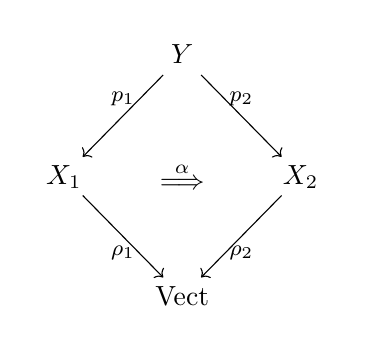
\begin{tikzpicture}[
			     baseline=(current bounding box.base), 
			     %>=stealth,
			     descr/.style={fill=white,inner sep=3.5pt}, 
			     normal line/.style={->}
			     ] 
\matrix (m) [matrix of math nodes, row sep=3.0em, column sep=2em, text height=1.5ex, text depth=0.1ex] {%
{} & Y & {} 
\\
X_1 & {} & X_2 
\\
{} & \Vect & {} 
\\
};
\path[font=\footnotesize] (m-1-2) edge[->] node[above] {$p_1$} (m-2-1);
\path[font=\footnotesize] (m-1-2) edge[->] node[above] {$p_2$} (m-2-3);
\path[font=\footnotesize] (m-2-1) edge[->] node[below] {$\rho_1$} (m-3-2);
\path[font=\footnotesize] (m-2-3) edge[->] node[below] {$\rho_2$} (m-3-2);
\fill (0,0) circle (0pt) node {$\stackrel{\alpha}{\implies}$};
\end{tikzpicture}
%%%%%%%%%%%%%%%%%%%%%%% 
\! , \quad 
%%%%%%%%%%%%%%%%%%%%%%%
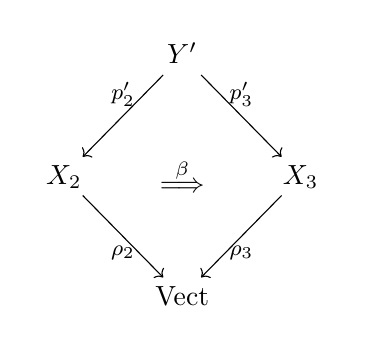
\begin{tikzpicture}[
			     baseline=(current bounding box.base), 
			     %>=stealth,
			     descr/.style={fill=white,inner sep=3.5pt}, 
			     normal line/.style={->}
			     ] 
\matrix (m) [matrix of math nodes, row sep=3.0em, column sep=2em, text height=1.5ex, text depth=0.1ex] {%
{} & Y' & {} 
\\
X_2 & {} & X_3 
\\
{} & \Vect & {} 
\\
};
\path[font=\footnotesize] (m-1-2) edge[->] node[above] {$p'_2$} (m-2-1);
\path[font=\footnotesize] (m-1-2) edge[->] node[above] {$p'_3$} (m-2-3);
\path[font=\footnotesize] (m-2-1) edge[->] node[below] {$\rho_2$} (m-3-2);
\path[font=\footnotesize] (m-2-3) edge[->] node[below] {$\rho_3$} (m-3-2);
\fill (0,0) circle (0pt) node {$\stackrel{\beta}{\implies}$};
\end{tikzpicture}
%%%%%%%%%%%%%%%%%%%%%%% 
\! .
$$%
Then by definition of $\textrm{Fam}_1(\Vect)$, their composition $\beta \circ_\eta \alpha$ is the natural transformation $(\beta * 1_{\pi_2}) \cdot (1_{\rho_2} * \eta) \cdot (\alpha * 1_{\pi_1})$: 
$$
\beta \circ_\eta \alpha 
\; \stackrel{\text{def}}{=} \; 
%%%%%%%%%%%%%%%%%%%%%%%
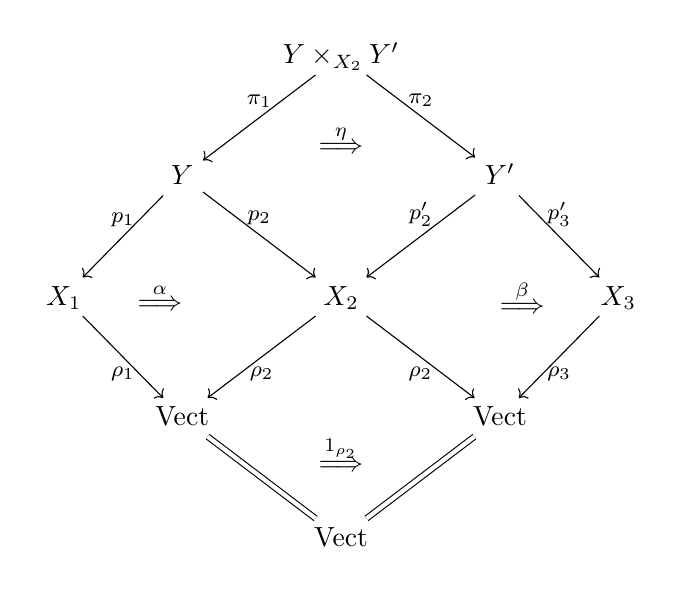
\begin{tikzpicture}[
			     baseline=(current bounding box.base), 
			     %>=stealth,
			     descr/.style={fill=white,inner sep=3.5pt}, 
			     normal line/.style={->}
			     ] 
\matrix (m) [matrix of math nodes, row sep=3.0em, column sep=2em, text height=1.5ex, text depth=0.1ex] {%
{} & {} & Y \times_{X_2} Y' & {} & {}
\\
{} & Y & {} & Y' & {}
\\
X_1 & {} & X_2 & {} & X_3
\\
{} & \Vect & {} & \Vect & {}
\\
{} & {} & \Vect & {} & {}
\\
};
\path[font=\footnotesize] (m-1-3) edge[->] node[above] {$\pi_1$} (m-2-2);
\path[font=\footnotesize] (m-1-3) edge[->] node[above] {$\pi_2$} (m-2-4);
\path[font=\footnotesize] (m-2-2) edge[->] node[above] {$p_1$} (m-3-1);
\path[font=\footnotesize] (m-2-2) edge[->] node[above] {$p_2$} (m-3-3);
\path[font=\footnotesize] (m-2-4) edge[->] node[above] {$p'_2$} (m-3-3);
\path[font=\footnotesize] (m-2-4) edge[->] node[above] {$p'_3$} (m-3-5);
\path[font=\footnotesize] (m-3-1) edge[->] node[below] {$\rho_1$} (m-4-2);
\path[font=\footnotesize] (m-3-3) edge[->] node[below] {$\rho_2$} (m-4-2);
\path[font=\footnotesize] (m-3-3) edge[->] node[below] {$\rho_2$} (m-4-4);
\path[font=\footnotesize] (m-3-5) edge[->] node[below] {$\rho_3$} (m-4-4);
\path[font=\footnotesize] (m-4-2) edge[commutative diagrams/equal] node[below] {} (m-5-3);
\path[font=\footnotesize] (m-4-4) edge[commutative diagrams/equal] node[below] {} (m-5-3);
%
\fill (-2.3,0) circle (0pt) node {$\stackrel{\alpha}{\implies}$};
\fill (2.3,0) circle (0pt) node {$\stackrel{\beta}{\implies}$};
\fill (0,2) circle (0pt) node {$\stackrel{\eta}{\implies}$};
\fill (0,-2) circle (0pt) node {$\stackrel{1_{\rho_2}}{\implies}$};
\end{tikzpicture}
%%%%%%%%%%%%%%%%%%%%%%% 
\! . 
$$
Furthermore, by definition of $\textrm{Sum}_1$, its action on the three morphisms is as follows: 
\begin{align*}
\textrm{Sum}_1(\alpha) & 
= {p_2}_* \cdot (\alpha\circ(-)) \cdot p_1^* \, , 
\\
\textrm{Sum}_1(\beta) & 
= {p'_3}_* \cdot (\beta\circ(-)) \cdot {p'_2}^* \, , 
\\
\textrm{Sum}_1(\beta \circ_\eta \alpha ) & 
= ({p'_3} \circ \pi_2)_* \cdot (\beta \circ_\eta \alpha \circ(-)) \cdot (p_1 \circ \pi_1)^* \, . 
\end{align*}

To show that $\textrm{Sum}_1(\beta \circ_\eta \alpha ) = \textrm{Sum}_1(\beta) \circ \textrm{Sum}_1(\alpha)$, we first observe that the left-hand side is the clock-wise composition of the outmost arrows from the top left to the bottom left vertex in the following diagram: 
$$
\!\!\!
%%%%%%%%%%%%%%%%%%%%%%%
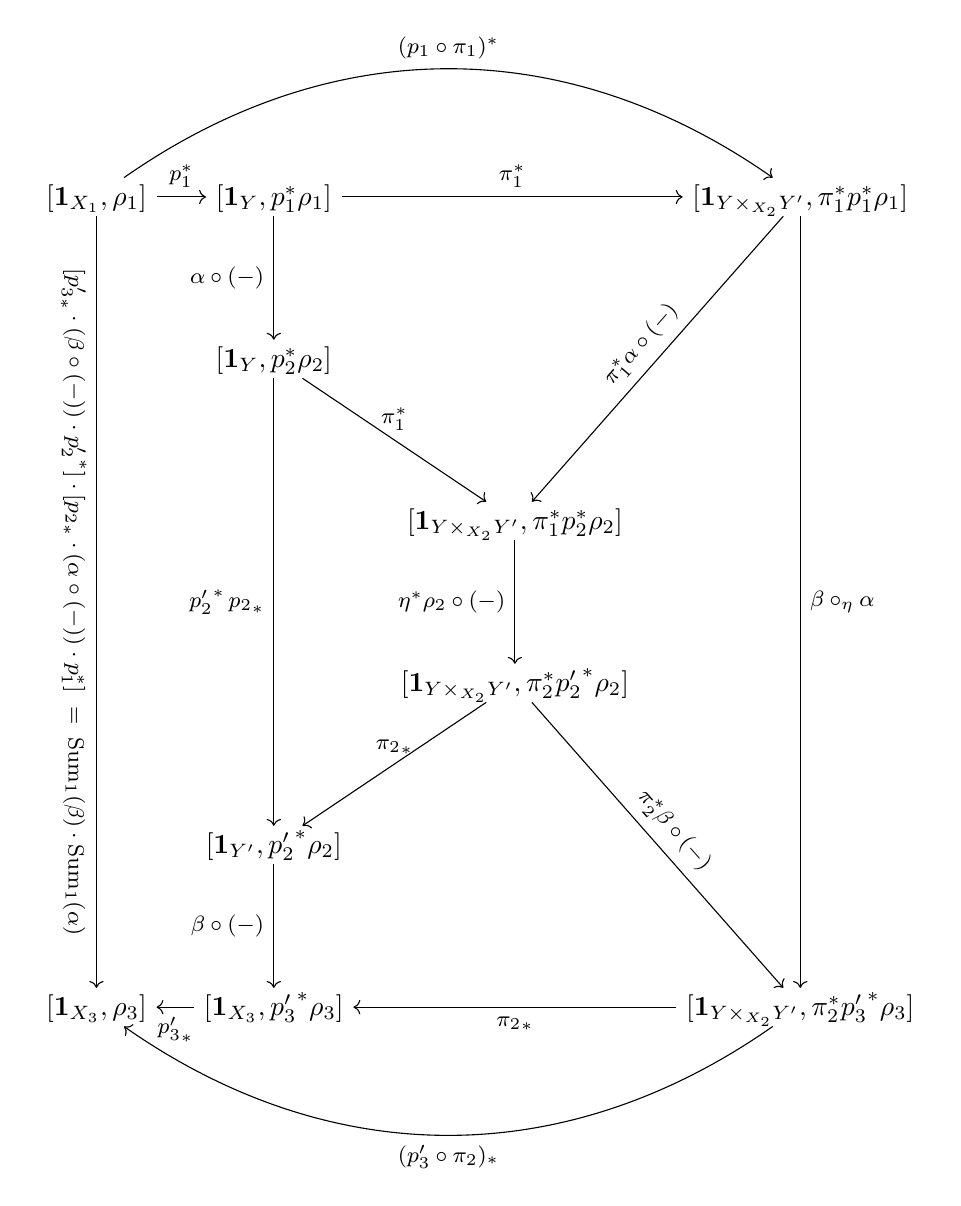
\begin{tikzpicture}[
			     baseline=(current bounding box.base), 
			     %>=stealth,
			     descr/.style={fill=white,inner sep=3.5pt}, 
			     normal line/.style={->}
			     ] 
\matrix (m) [matrix of math nodes, row sep=4.5em, column sep=1.4em, text height=1.5ex, text depth=0.1ex] {%
[\mathbf{1}_{X_1},\rho_1]  &  {}[\mathbf{1}_{Y}, p^*_1\rho_1]   &  {}  &   {}[\mathbf{1}_{Y \times_{X_2} Y'}, \pi_1^* p_1^*\rho_1]
\\
  & {}[\mathbf{1}_{Y}, p_2^*\rho_2] & {} & 
\\
  & {} & {}[\mathbf{1}_{Y \times_{X_2} Y'}, \pi_1^* p_2^* \rho_2] & 
\\
  & {} & {}[\mathbf{1}_{Y \times_{X_2} Y'}, \pi_2^* {p'_2}^* \rho_2] & 
\\
  & {}[\mathbf{1}_{Y'}, {p'_2}^* \rho_2] & {} & 
\\
{}[\mathbf{1}_{X_3},\rho_3]  &  {}[\mathbf{1}_{X_3}, {p'_3}^* \rho_3]   &  {}  &  {}[\mathbf{1}_{Y \times_{X_2} Y'}, \pi_2^* {p'_3}^*\rho_3]
\\
};
\path[font=\footnotesize] (m-1-1) edge[->, out= 35, in= 145] node[sloped, above] {$(p_1\circ \pi_1)^*$} (m-1-4);
\path[font=\footnotesize] (m-1-1) edge[->] node[above] {$p_1^*$} (m-1-2);
\path[font=\footnotesize] (m-1-2) edge[->] node[above] {$\pi_1^*$} (m-1-4);
\path[font=\footnotesize] (m-1-2) edge[->] node[left] {$\alpha\circ(-)$} (m-2-2);
\path[font=\footnotesize] (m-2-2) edge[->] node[above] {$\pi_1^*$} (m-3-3);
\path[font=\footnotesize] (m-2-2) edge[->] node[left] {${p'_2}^* \, {p_2}_*$} (m-5-2);
\path[font=\footnotesize] (m-1-4) edge[->] node[sloped, above] {$\pi_1^*\alpha\circ(-)$} (m-3-3);
\path[font=\footnotesize] (m-1-4) edge[->] node[right] {$\beta \circ_\eta \alpha$} (m-6-4);
\path[font=\footnotesize] (m-3-3) edge[->] node[left] {$\eta^*\rho_2 \circ (-)$} (m-4-3);
\path[font=\footnotesize] (m-4-3) edge[->] node[above] {${\pi_2}_*$} (m-5-2);
\path[font=\footnotesize] (m-4-3) edge[->] node[sloped, above] {$\pi_2^*\beta\circ(-)$} (m-6-4);
\path[font=\footnotesize] (m-5-2) edge[->] node[left] {$\beta\circ(-)$} (m-6-2);
\path[font=\footnotesize] (m-6-4) edge[->] node[below] {${\pi_2}_*$} (m-6-2);
\path[font=\footnotesize] (m-6-2) edge[->] node[below] {${p'_3}_*$} (m-6-1);
\path[font=\footnotesize] (m-1-1) edge[->] node[sloped, below] {$[{p'_3}_* \cdot (\beta\circ(-)) \cdot {p'_2}^*] \cdot [{p_2}_* \cdot (\alpha\circ(-)) \cdot p_1^*] \; = \; \text{Sum}_1(\beta) \cdot \text{Sum}_1 (\alpha)$} (m-6-1);
\path[font=\footnotesize] (m-6-4) edge[->, out= -145, in= -35] node[sloped, below] {$(p'_3\circ \pi_2)_*$} (m-6-1);
\end{tikzpicture}
%%%%%%%%%%%%%%%%%%%%%%% 
$$
The leftmost vertical arrow is $\textrm{Sum}_1(\beta) \circ \textrm{Sum}_1(\alpha)$, hence we are done if we can show that the diagram commutes. 
This is indeed the case: 
the leftmost and rightmost subdiagrams commute by definition, as does the other subdiagram involving $\pi_1^*\alpha\circ(-)$; 
that the top and bottom diagrams commute follows from the definition of pullback and pushforward; 
finally, the subdiagram involving $\pi_2^*\beta\circ(-)$ and ${\pi_2}_*$ commutes by the projection formula of Lemma~\ref{lem:projectionformula}, 
and the middle subdiagram commutes thanks to the Beck-Chevalley condition of Lemma~\ref{lem:BeckChevalley}. 

Finally, if $\rho_2=\rho_3$, $Y=Y'$ and $\beta$ is the identity on $\rho_2$ in $\textrm{Fam}_1(\Vect)$, then $Y \times_{X_2} Y'$ is canonically equivalent to~$Y$, and we see that $\textrm{Sum}_1$ sends units to units. 
\end{proof}


\subsection[$n=2$]{$\boldsymbol{n=2}$}

\subsubsection{``Without thinking'' (Nils)}

Now let $\omega \in Z^2(G,\C^\times)$. 
We will construct a 2-functor 
\be
\label{eq:TQFTfactored2}
%%%%%%%%%%%%%%%%%%%%%%%
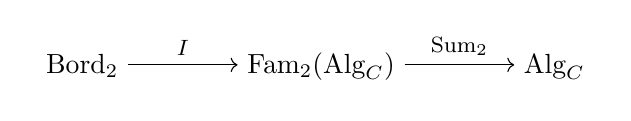
\begin{tikzpicture}[
			     baseline=(current bounding box.base), 
			     %>=stealth,
			     descr/.style={fill=white,inner sep=3.5pt}, 
			     normal line/.style={->}
			     ] 
\matrix (m) [matrix of math nodes, row sep=3.5em, column sep=4.0em, text height=1.5ex, text depth=0.1ex] {%
\Bord_2  &  \textrm{Fam}_2(\text{Alg}_\C)  &  \text{Alg}_\C 
\\
};
\path[font=\footnotesize] (m-1-1) edge[->] node[above] {$I$} (m-1-2);
\path[font=\footnotesize] (m-1-2) edge[->] node[above] {$\textrm{Sum}_2$} (m-1-3);
\end{tikzpicture}
%%%%%%%%%%%%%%%%%%%%%%% 
\ee
by computing what it does to $\text{pt}_+ \in \Bord_2$. 
The first step is to set $I(\text{pt}_+)$ to be the 2-functor 
\begin{align}
\chi^\omega \colon \boldB G 
& \lra \Algc  
&& \text{with} \quad \chi^\omega_{g,h} := \omega(g,h) \colon L_g \otimes_\C L_h \to L_{gh}
\label{eq:chiomega2}
\\
* & \lmt \C && \nonumber
\\
G \ni g & \lmt L_g := {}_\C \C_\C && \nonumber && \nonumber
\\
1_g & \lmt  1_\C && \nonumber
\end{align}
(Recall from \cite[Sect.\,1.1]{LeinsterBasic2} that the constraint on the coherence 2-morphisms $\chi^\omega_{g,h} = \omega(g,h) \in \End_\C(\C)$ is precisely the 2-cocycle condition on~$\omega$. 
Also note that all our 2-functors are strictly unital, so in particular~\eqref{eq:chiomega2} completely specifies the 2-functor~$\chi^\omega$.) 

The second step is to compute the 2-colimit $\text{Sum}_2(\chiom)$. 
There are several versions of 2-limit, bilimit, weighted bilimit etc.~in the literature.  
We will use the notion of \cite[Def.\,7.4.4]{bor94} and call it 2-limit. 
To give the details, recall the definitions from \cite[Sect.\,1.2--3]{LeinsterBasic2}, and that the \textsl{opposite} $\B^{\text{op}}$ of a bicategory~$\B$ has reversed horizontal composition, but the same vertical composition as~$\B$. 

\begin{definition}
\label{def:2limit}
Let $F \colon \mathcal A \to \B$ be a 2-functor, and let $B\in\B$. 
\begin{enumerate}
\item
The \textsl{constant 2-functor} $\Delta_B \colon \mathcal A \to \B$ sends every object in~$\mathcal A$ to~$B$, 1- and 2-morphisms in~$\mathcal A$ to $1_B$ and $1_{1_B}$, respectively, and all constraints $(\Delta_B)_{g,h}$ are trivial. 
\item 
The category $2\text{-Cone}(B,F)$ of \textsl{2-cones on~$F$ with vertex~$B$} is the category whose objects are pseudonatural transformations $\Delta_B \to F$ and whose morphisms are modifications between them. 
\item 
A \textsl{2-limit} of~$F$ is a pair $(L,\pi)$ with $L\in \B$ and $\pi \colon \Delta_L \to F$ a pseudonatural transformation such that the functor
\begin{align*}
%\pi_* \colon 
\B(B,L) 
& \lra 2\text{-Cone}(B,F) 
\\
(B \stackrel{f}{\lra} L) 
& \lmt (\Delta_B \stackrel{f_*}{\lra} \Delta_L \stackrel{\pi}{\lra} F) 
\end{align*}
is an equivalence of categories for all $B\in\B$. 
\item 
Now let $G \colon \mathcal A \to \B^{\text{op}}$. 
The category $2\text{-Cocone}(B,G)$ of \textsl{2-cocones on~$G$ with vertex $B \in \B$} is defined to be $2\text{-Cone}(B,G)$, but with~$B$ viewed as an object in $\B^{\text{op}}$. 
A 2-limit of $G \colon \mathcal A \to \B^{\text{op}}$ is also called a \textsl{2-colimit of~$G$ in~$\B$}. 
\end{enumerate}
\end{definition}

Spelling out the definition, we see that an object $\sigma \colon \Delta_B \to F$ of $2\text{-Cone}(B,F)$ is a family of 1- and 2-morphisms 
\be
\label{eq:2cone1}
\big\{ B \stackrel{\sigma_A}{\lra} F(A) \big\}_{A\in\mathcal A}
\quad\text{ and }\quad 
\big\{ F(g) \otimes \sigma_A \stackrel{\sigma_g}{\lra} \sigma_{A'} \big\}_{g\in\mathcal A(A,A')}
\ee
such that 
\be
\label{eq:2cone2}
%%%%%%%%%%%%%%%%%%%%%%%
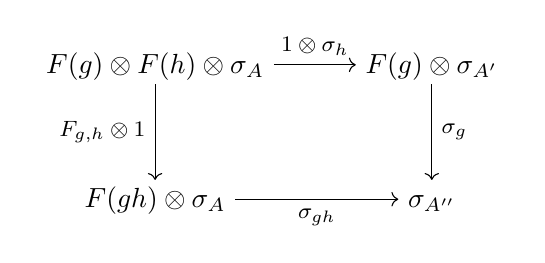
\begin{tikzpicture}[
			     baseline=(current bounding box.base), 
			     %>=stealth,
			     descr/.style={fill=white,inner sep=3.5pt}, 
			     normal line/.style={->}
			     ] 
\matrix (m) [matrix of math nodes, row sep=3.5em, column sep=3.0em, text height=1.5ex, text depth=0.1ex] {%
F(g) \otimes F(h) \otimes \sigma_A  &  F(g) \otimes \sigma_{A'}
\\
F(gh) \otimes \sigma_A  & \sigma_{A''}
\\
};
\path[font=\footnotesize] (m-1-1) edge[->] node[above] {$1\otimes \sigma_h$} (m-1-2);
\path[font=\footnotesize] (m-1-1) edge[->] node[left] {$F_{g,h} \otimes 1$} (m-2-1);
\path[font=\footnotesize] (m-2-1) edge[->] node[below] {$\sigma_{gh}$} (m-2-2);
\path[font=\footnotesize] (m-1-2) edge[->] node[right] {$\sigma_{g}$} (m-2-2);
\end{tikzpicture}
%%%%%%%%%%%%%%%%%%%%%%% 
\ee
commutes for all 
$
A \stackrel{h}{\lra} A' \stackrel{g}{\lra} A''
$. 
Furthermore, a morphism $\Gamma \colon \sigma \to \widetilde\sigma$ in $2\text{-Cone}(B,F)$ is a family 
\be
\label{eq:2cone3}
\big\{ \sigma_A \stackrel{\Gamma_A}{\lra} \widetilde\sigma_A \big\}_{A\in\mathcal A}
\quad\text{ such that }\quad 
%%%%%%%%%%%%%%%%%%%%%%%
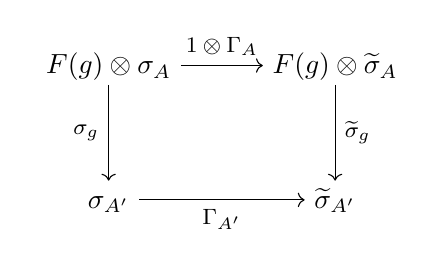
\begin{tikzpicture}[
			     baseline=(current bounding box.base), 
			     %>=stealth,
			     descr/.style={fill=white,inner sep=3.5pt}, 
			     normal line/.style={->}
			     ] 
\matrix (m) [matrix of math nodes, row sep=3.5em, column sep=3.0em, text height=1.5ex, text depth=0.1ex] {%
F(g) \otimes \sigma_A  &  F(g) \otimes \widetilde\sigma_A
\\
\sigma_{A'}  & \widetilde\sigma_{A'}
\\
};
\path[font=\footnotesize] (m-1-1) edge[->] node[above] {$1\otimes \Gamma_A$} (m-1-2);
\path[font=\footnotesize] (m-1-1) edge[->] node[left] {$\sigma_g$} (m-2-1);
\path[font=\footnotesize] (m-2-1) edge[->] node[below] {$\Gamma_{A'}$} (m-2-2);
\path[font=\footnotesize] (m-1-2) edge[->] node[right] {$\widetilde\sigma_{g}$} (m-2-2);
\end{tikzpicture}
%%%%%%%%%%%%%%%%%%%%%%% 
\ee
commutes for all 
$
A \stackrel{g}{\lra} A'
$. 

Note that above ``$\otimes$'' is exclusively used for the horizontal composition in the target~$\B$ (while juxtaposition is used for the horizontal composition in~$\mathcal A$). 
Hence going to $\B^{\text{op}}$ amounts to reversing all the tensor products above. 

\begin{lemma}
\label{lem:2cone}
Let $B\in \Algc$ and $\chiom \colon \boldB G \to \Algc$ as in~\eqref{eq:chiomega2}. 
Then 
\begin{align}
2\text{-Cone}(B,\chiom) & \cong  {}_{\CGtw}\text{Mod}_B \, , \nonumber 
\\
2\text{-Cocone}(B,\chiom) & \cong  {}_{B}\text{Mod}_{\CGtw}
\end{align}
where $\CGtw$ is the $\omega$-twisted group algebra of~$G$. 
\end{lemma}

\begin{proof}
We only prove the the statement about 2-cones in detail, the one about 2-cocones follows analogously by reversing all horizontal compositions in~$\B$. 

By \eqref{eq:2cone1} and \eqref{eq:2cone2}, an object in $2\text{-Cone}(B,\chiom)$ is a 1-morphism $M \in \Algc(B,\C)$ together with linear maps $\sigma_g \colon L_g \otimes_\C M \to M$ such that 
\be
%%%%%%%%%%%%%%%%%%%%%%%
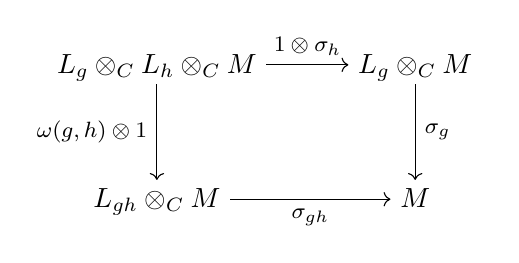
\begin{tikzpicture}[
			     baseline=(current bounding box.base), 
			     %>=stealth,
			     descr/.style={fill=white,inner sep=3.5pt}, 
			     normal line/.style={->}
			     ] 
\matrix (m) [matrix of math nodes, row sep=3.5em, column sep=3.0em, text height=1.5ex, text depth=0.1ex] {%
L_g \otimes_\C L_h \otimes_\C M  &  L_g \otimes_\C M
\\
L_{gh} \otimes_\C M  & M
\\
};
\path[font=\footnotesize] (m-1-1) edge[->] node[above] {$1\otimes \sigma_h$} (m-1-2);
\path[font=\footnotesize] (m-1-1) edge[->] node[left] {$\omega(g,h) \otimes 1$} (m-2-1);
\path[font=\footnotesize] (m-2-1) edge[->] node[below] {$\sigma_{gh}$} (m-2-2);
\path[font=\footnotesize] (m-1-2) edge[->] node[right] {$\sigma_{g}$} (m-2-2);
\end{tikzpicture}
%%%%%%%%%%%%%%%%%%%%%%% 
\ee
commutes for all $g,h \in G$. 
But this means that $(M, \sum_{g\in G} \sigma_g$) is a left $\CGtw$-module, while by definition of $\Algc$, the 1-morphism $M \in \Algc(B,\C)$ is a right $B$-module. 

According to \eqref{eq:2cone3}, a morphism $(M, \{ \sigma_g \}) \to (\widetilde M, \{ \widetilde\sigma_g \})$ in $2\text{-Cone}(B,\chiom)$ is a 2-morphism $\Gamma \colon {}_\C M_B \to {}_\C \widetilde M_B$ in $\Algc$ such that 
\be
%%%%%%%%%%%%%%%%%%%%%%%
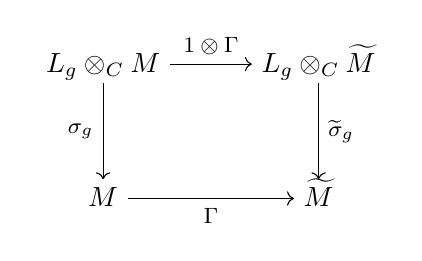
\begin{tikzpicture}[
			     baseline=(current bounding box.base), 
			     %>=stealth,
			     descr/.style={fill=white,inner sep=3.5pt}, 
			     normal line/.style={->}
			     ] 
\matrix (m) [matrix of math nodes, row sep=3.5em, column sep=3.0em, text height=1.5ex, text depth=0.1ex] {%
L_g \otimes_\C M  &  L_g \otimes_\C \widetilde M
\\
M  & \widetilde M
\\
};
\path[font=\footnotesize] (m-1-1) edge[->] node[above] {$1\otimes \Gamma$} (m-1-2);
\path[font=\footnotesize] (m-1-1) edge[->] node[left] {$\sigma_g$} (m-2-1);
\path[font=\footnotesize] (m-2-1) edge[->] node[below] {$\Gamma$} (m-2-2);
\path[font=\footnotesize] (m-1-2) edge[->] node[right] {$\widetilde\sigma_{g}$} (m-2-2);
\end{tikzpicture}
%%%%%%%%%%%%%%%%%%%%%%% 
\ee 
commutes. 
But that means that~$\Gamma$ is both a map of left $\CGtw$-modules and a map of right $B$-modules. 
\end{proof}

\begin{proposition}
\begin{enumerate}
\item
A 2-limit of $\chiom \colon \boldB G \to \Algc$ is given by $(\CGtw, \CGtw)$. 
\item
A 2-colimit of $\chiom \colon \boldB G \to \Algc$ is given by $(\CGtw, \CGtw)$. 
\end{enumerate}
\end{proposition}

\begin{proof}
According to Definition~\ref{def:2limit} and Lemma~\ref{lem:2cone}, a 2-limit of $\chiom$ is an algebra $L \in \Algc$ together with a module ${}_{\CGtw} M_L$ such that the functor 
\begin{align*}
\Algc(B,L) 
& \lra {}_{\CGtw}\text{Mod}_B
\\
N & \lmt M \otimes_L N
\end{align*}
is an equivalence for every $B \in \Algc$. 
This is the case for $L = \CGtw$ as an algebra and $M = \CGtw$ as a bimodule over itself. 

The statement about the 2-colimit follows analogously. 
\end{proof}


\subsubsection{``With thinking'' (Domenico)}

The datum of the 2-functor $\chi^\omega \colon \boldB G \to \text{Alg}_\C$ is a collection of lines (1-dimensional complex vector spaces) $L_g$, indexed by elements in the group $G$, together with isomorphisms
\[
\rho_{g,h}\colon L_g\otimes L_h\xrightarrow{\sim} L_{gh}
\]
subject to the associativity constraint given by the commutativity of the diagrams
\[
\xymatrix{
L_g\otimes L_h\otimes L_k\ar[rr]^{\rho_{g,h}\otimes \mathrm{id}}\ar[d]_{\mathrm{id}\otimes \rho_{h,k}}&& L_{gh}\otimes L_k\ar[d]^{\rho_{gh,k}}\\
L_g\otimes L_{hk}\ar[rr]_{\rho_{g,hk}} &&L_{ghk}
}
\]
where the tensor products are over $\C$. We also require that $L_1=\C$ and that the isomorphisms $L_1\otimes L_g\xrightarrow{\sim}L_g$ and $L_g\otimes L_1\xrightarrow{\sim}L_g$ are the structure isomorphisms for the unit object $\C$ of the monoidal category $\mathrm{Vect}_\C$.
The associativity constraints imply, and are in fact equivalent to this, that the vector space
\[
A_{\chi^\omega}=\bigoplus_{g\in G} L_g
\]
has an associative $\C$-algebra structure.
\begin{lemma}
A choice of a basis element $x_g$ for every line $L_g$ defines a $\C^\times$-valued 2-cocycle $\omega$ on the group $G$. A different choice of basis elements leads to a cohomologous cocycle, so that the class $[\omega]\in H^2(G,\C^\times)$ is well defines.
\end{lemma}
\begin{proof}
As $\rho_{g,h}(x_g\otimes x_h)$ is a nonzero element in $L_{gh}$ we have $\rho_{g,h}(x_g\otimes x_h)=\omega(g,h)x_{gh}$ for a unique element $\omega(g,h)$ in $\C^\times$. The associativity constraints are then immediately seen to be equivalent to the cocycle equation
\[
\omega(gh,k)\omega(g,h)=\omega(g,hk)\omega(h,k).
\]
Finally, if $\{y_g\}_{g\in G}$ is a different basis choice, and $\tilde{\omega}$ is the corresponding 2-cocycle, then we have $y_g=\eta_gx_g$ for some $\eta_g$ in $\C^\times$ and
\[
\tilde{\omega(g,h)}y_{gh}=\rho_{g,h}(y_g\otimes y_h)=\eta_g\eta_h\rho_{g,h}(x_g\otimes x_h)=\eta_g\eta_h\omega(g,h)x_{gh}=\eta_g\eta_h\omega(g,h)\eta_{gh}^{-1}y_{gh}.
\]
Therefore
\[
\tilde{\omega}(g,h)=\eta_g\eta_{gh}^{-1}\eta_h\omega(g,h),
\]
i.e. $\omega$ and $\tilde{\omega}$ are cohomologous.
\end{proof}
\begin{corollary}
The algebra $A_{\chi^\omega}$ is isomorphic to the twisted group algebra $\C^\omega[G]$, defined as the $\C$-vector space on the basis $\{x_g\}_{g\in G}$ with the product $x_g\cdot x_h=\omega(g,h)x_{gh}$ and with $x_1=1$.
\end{corollary}
\begin{lemma}\label{lemma:cocone-is-coinvariants}
$\text{Sum}_2(\chi^\omega) \cong \C^\omega[G]$, the  twisted group algebra of $G$.
\end{lemma}

\begin{proof}
Let $(A,M)$ be a cocone for $\chi^\omega$, i.e., a pair consisting of a $\C$-algebra $A$ together with a left $A$-module $M$ (representing a linear functor ${}_\C\mathrm{Mod}\to {}_A\mathrm{Mod}$) and homotopy commutative diagrams
\[
\xymatrix{
&A\\
\C\ar[rr]_{L_g}\ar[ur]^{M}&&\C\ar[lu]_M
\ar@{=>}^{\lambda_g}(18,-11);(9,-6)}
\]
where the $\lambda_g$'s are isomorphisms of left $A$-modules
\[
\lambda_g\colon  M\otimes_\C L_g\xrightarrow{\sim} M
\]
such that the diagrams
\[
\xymatrix{
M\otimes L_g\otimes L_h\ar[rr]^{\lambda_{g}\otimes \mathrm{id}}\ar[d]_{\mathrm{id}\otimes \rho_{g,h}}&& M\otimes L_h\ar[d]^{\lambda_h}\\
M\otimes L_{gh}\ar[rr]_{\lambda_{gh}} &&M
}
\]
commute. This implies that the isomorphisms $\lambda_g$ make $M$ a right $A_{\chi^\omega}$-module. Therefore, we can see $M$ as a linear functor 
\[
{}_{A_{\chi^\omega}}\mathrm{Mod}\to {}_A\mathrm{Mod}
\]
i.e., as a morphism from $A_{\chi^\omega}$ to $A$ in $2\text{-}\mathrm{Vect}_\C$. The algebra $A_{\chi^\omega}$ seen as a left $A_{\chi^\omega}$-module is a morphism from $\C$ to $A_{\chi^\omega}$ in $2\text{-}\mathrm{Vect}_\C$ and the natural isomorphism
\[
{}_AM_\C\cong {}_AM_{A_{\chi^\omega}}\otimes {}_{A_{\chi^\omega}}{A_{\chi^\omega}}_\C
\]
gives a canonical factorization
\[
\xymatrix{
&A\\
&A_{\chi^\omega}\ar[u]^{M}\\
\C\ar[rr]_{L_g}\ar[ur]^{A_{\chi^\omega}}\ar@/^2pc/[ruu]^{M}&&\C\ar[lu]_{A_{\chi^\omega}}\ar@/_2pc/[luu]_{M}
\ar@{=>}^{\lambda_g}(15,-26);(22,-21)}
\]
exhibiting the algebra $A_{\chi^\omega}$ together with itself seen as a left module over itself as the universal cocone. 
\end{proof}


\subsection[$n=3$]{$\boldsymbol{n=3}$}

TODO:
\begin{itemize}
\item
The only non-trivial part of the 3-functor $\chi^\omega \colon \boldB G \to \text{TC}_\C$ are the coherence 3-morphisms which assemble into the modification (also) called~$\omega$ in \cite[Def.\,A.4.3]{GregorDiss}, and the constraints on $\omega$ (see \cite[Page~219]{GregorDiss}) seem to be precisely the 3-cocycle condition. 
\item
\underline{\textbf{Issue}}: The notion of a 3-colimit (to really compute $\text{Sum}_3$) is scary. 
At least we should make some hand-wavy arguments\dots
\end{itemize}


\section{Boundary conditions}

\subsection[$n=2$]{$\boldsymbol{n=2}$}

TODO

\subsection[$n=3$]{$\boldsymbol{n=3}$}

TODO






\begin{thebibliography}{BDSPV}

\bibitem[Bo]{bor94}
F.~Borceux, 
\textsl{Handbook of categorical algebra 1}, 
volume 50 of \textsl{Encyclopedia of Mathematics and its Applications}, 
Cambridge University Press, Cambridge, 1994.

\bibitem[FHLT]{FHLT}
D.~Freed, M.~Hopkins, J.~Lurie, and C.~Teleman,
\textsl{Topological Quantum Field Theories from Compact Lie Groups}, 
\href{http://arxiv.org/abs/0905.0731}{[\mbox{arXiv:}0905.0731]}. 

\bibitem[Le]{LeinsterBasic2}
T.~Leinster, 
\textsl{Basic Bicategories}, 
\href{http://arxiv.org/abs/math/9810017}{[math/9810017]}.

\bibitem[Lu]{l0905.0465}
J.~Lurie, 
\textsl{On the Classification of Topological Field Theories},
\href{https://projecteuclid.org/euclid.cdm/1254748657}{Current Developments in Mathematics \textbf{2008} (2009), 129--280}, 
\arxiv{0905.0465}{[arXiv:0905.0465]}.

\bibitem[Sc]{GregorDiss}
G.~Schaumann, 
\textsl{Duals in tricategories and in the tricategory of bimodule categories}, 
PhD thesis, 
Friedrich-Alexander-Universit\"at Erlangen-N\"urnberg (2013), 
% \url{http://opus4.kobv.de/opus4-fau/frontdoor/index/index/docId/3732}.
%\newline
%\href{http://opus4.kobv.de/opus4-fau/frontdoor/index/index/docId/3732}{http://opus4.kobv.de/opus4-fau/frontdoor/index/index/docId/3732}.
\href{http://nbn-resolving.de/urn/resolver.pl?urn:nbn:de:bvb:29-opus4-37321}{urn:nbn:de:bvb:29-opus4-37321}.

\bibitem[Wi]{WittenParity2016}
E.~Witten, 
\textsl{The ``Parity'' Anomaly On An Unorientable Manifold}, 
\href{http://arxiv.org/abs/1605.02391}{[arXiv:1605.02391]}.  

\bibitem[WWW]{WWW}
J.~Wang, X.-G.~Wen and E.~Witten, 
\textsl{Symmetric Gapped Interfaces of SPT and SET States: Systematic Constructions}, 
\href{http://arxiv.org/abs/1705.06728}{[arXiv:1705.06728]}.  




\end{thebibliography}



\end{document}

